\documentclass[12pt, a4paper]{article}

\usepackage{fontspec}
\usepackage{polyglossia}

\setmainlanguage{russian}
\setotherlanguages{english}

% download "Linux Libertine" OTF-fonts:
% http://www.linuxlibertine.org/index.php?id=91&L=1
\setmainfont{Linux Libertine O} % or Helvetica, Arial, Cambria
% why do we need \newfontfamily:
% http://tex.stackexchange.com/questions/91507/
\newfontfamily{\cyrillicfonttt}{Linux Libertine O}
\newfontfamily{\cyrillicfont}{Linux Libertine O}
\newfontfamily{\cyrillicfontsf}{Linux Libertine O}

\usepackage{etoolbox} % to use ifdef, must be after babel

\usepackage[paper=a4paper,
top=13.5mm, bottom=13.5mm,
left=16.5mm, right=13.5mm, includefoot]{geometry}

\usepackage{etex} % расширение классического tex
% в частности позволяет подгружать гораздо больше пакетов, чем мы и займёмся далее




\usepackage{makeidx} % для создания предметных указателей
\usepackage{verbatim} % для многострочных комментариев
%\usepackage[pdftex]{graphicx} % для вставки графики
% omit pdftex option if not using pdflatex


%\usepackage{dsfont} % шрифт для единички с двойной палочкой (для индикатора события)
\usepackage{bbm} % шрифт - двойные буквы


\usepackage[usenames, dvipsnames, svgnames, table, rgb]{xcolor}

\usepackage{colortbl}


% пакет для тестов:
\usepackage[box, % запрет на перенос вопросов
nopage, % убираем колонтитулы страницы
insidebox, % ставим буквы в квадратики
separateanswersheet, % добавляем бланк ответов
nowatermark, % отсутствие надписи "Черновик"
%indivanswers,  % показываем верные ответы
%answers,
lang=RU, % локализация слов "нет верных ответов", "вопрос" и тд
completemulti % добавлять "нет правильного ответа" во всех вопросах множественного выбора
]{automultiplechoice}


\usepackage{multicol}

\usepackage[colorlinks, hyperindex, unicode, breaklinks]{hyperref} % гиперссылки в pdf


\usepackage{amssymb}
\usepackage{amsmath}
\usepackage{amsthm}
\usepackage{epsfig}
\usepackage{bm}
\usepackage{color}



\usepackage{multirow} % Слияние строк в таблице

\usepackage{textcomp}  % Чтобы в формулах можно было русские буквы писать через \text{}

%\usepackage{embedfile} % Чтобы код LaTeXа включился как приложение в PDF-файл

\usepackage{subfigure} % для создания нескольких рисунков внутри одного

\usepackage{tikz, pgfplots} % язык для рисования графики из latex'a
\usetikzlibrary{trees} % прибамбас в нем для рисовки деревьев
\usetikzlibrary{arrows} % прибамбас в нем для рисовки стрелочек подлиннее
\usepackage{tikz-qtree} % прибамбас в нем для рисовки деревьев






\usepackage{enumitem}


%\embedfile[desc={Исходный LaTeX файл}]{\jobname.tex} % Включение кода в выходной файл
%\embedfile[desc={Стилевой файл}]{title_bor_utf8.tex}



% вместо горизонтальной делаем косую черточку в нестрогих неравенствах
\renewcommand{\le}{\leqslant}
\renewcommand{\ge}{\geqslant}
\renewcommand{\leq}{\leqslant}
\renewcommand{\geq}{\geqslant}

% делаем короче интервал в списках
\setlength{\itemsep}{0pt}
\setlength{\parskip}{0pt}
\setlength{\parsep}{0pt}

% свешиваем пунктуацию (т.е. знаки пунктуации могут вылезать за правую границу текста, при этом текст выглядит ровнее)
\usepackage{microtype}

% более красивые таблицы
\usepackage{booktabs}
% заповеди из докупентации:
% 1. Не используйте вертикальные линни
% 2. Не используйте двойные линии
% 3. Единицы измерения - в шапку таблицы
% 4. Не сокращайте .1 вместо 0.1
% 5. Повторяющееся значение повторяйте, а не говорите "то же"

\usepackage{minted} % вставка кода, нужен питон :)


\DeclareMathOperator{\grad}{grad}
\DeclareMathOperator{\card}{card}
\DeclareMathOperator{\sgn}{sign}
\DeclareMathOperator{\sign}{sign}

\DeclareMathOperator*{\argmin}{arg\,min}
\DeclareMathOperator*{\argmax}{arg\,max}
\DeclareMathOperator*{\amn}{arg\,min}
\DeclareMathOperator*{\amx}{arg\,max}
\DeclareMathOperator{\cov}{Cov}
\DeclareMathOperator{\Var}{Var}
\DeclareMathOperator{\Cov}{Cov}
\DeclareMathOperator{\Corr}{Corr}
\DeclareMathOperator{\E}{\mathbb{E}}
\let\P\relax
\DeclareMathOperator{\P}{\mathbb{P}}




\def \R{\mathbb{R}}
\def \N{\mathbb{N}}
\def \Z{\mathbb{Z}}





\newcommand{\dx}[1]{\,\mathrm{d}#1} % для интеграла: маленький отступ и прямая d
\newcommand{\ind}[1]{\mathbbm{1}_{\{#1\}}} % Индикатор события
%\renewcommand{\to}{\rightarrow}
\newcommand{\eqdef}{\mathrel{\stackrel{\rm def}=}}
\newcommand{\iid}{\mathrel{\stackrel{\rm i.\,i.\,d.}\sim}}
\newcommand{\const}{\mathrm{const}}


\usepackage{epigraph}

\AddEnumerateCounter{\asbuk}{\russian@alph}{щ} % для списков с русскими буквами
\setlist[enumerate, 2]{label=\asbuk*),ref=\asbuk*}




% \newenvironment{problem}{}{}
% тут перещёлкиваем комментарий, чтобы убрать или показать решения:
% \newenvironment{sol}{}{} % with solutions
% \excludecomment{sol} % without solutions



\unitlength=0.6mm

\title{Подборка экзаменов по теории вероятностей. \\Факультет экономики, НИУ ВШЭ}
\date{\today}
\author{Коллектив кафедры \\
математической экономики и эконометрики,
талантливые студенты,\\
 фольклор}


%%%%%%%%%%%%%%%%%% вставки
%%%%%%%%%%%%%%%%%%%%%%%%%%%%%%%%%%%%%%% Списки без уродских отступов
\newenvironment{enumerate*}{
\begin{enumerate}
  \setlength{\itemsep}{0pt}
  \setlength{\parskip}{0pt}
  \setlength{\parsep}{0pt}
}{\end{enumerate}}

\newenvironment{itemize*}{
\begin{itemize}
  \setlength{\itemsep}{0pt}
  \setlength{\parskip}{0pt}
  \setlength{\parsep}{0pt}
}{\end{itemize}}

\abovedisplayskip=0mm
\abovedisplayshortskip=0mm
\belowdisplayskip=0mm
\belowdisplayshortskip=0mm

% \newcommand{\MIN}{\textbf{(MIN)}{}}


\DeclareMathOperator{\Lin}{\mathrm{Lin}}
\DeclareMathOperator{\Linp}{\Lin^{\perp}}
\DeclareMathOperator*\plim{plim}
\newcommand{\cN}{\mathcal{N}}


\setcounter{secnumdepth}{0} % убираем нумерацию секций, подсекций и т.д.

\begin{document}
\maketitle

\tableofcontents{}


\parindent=0 pt % no indent

\section{Описание}

Свежую версию можно скачать с github-репозитория \url{https://github.com/bdemeshev/probability_hse_exams}.


Уникальное предложение для студентов факультета экономики НИУ-ВШЭ:


Найдите ошибки в этом документе или пришлите отсутствующие решения в техе и получите дополнительные бонусы!
Найденные смысловые ошибки поощряются сильнее, чем просто опечатки.
Замеченные ошибки и новые решения оформляйте в виде запросов на
\url{https://github.com/bdemeshev/probability_hse_exams/issues/}.
Перед публикацией запроса, пожалуйста, свертесь со свежей версией подборки.

В создании подборки храбро участвовали
Андрей Зубанов, Кирилл Пономарёв, Александр Левкун, Оля Гнилова,
Настя Жаркова, Гарик Варданян и другие :)


\subsection*{Доброе напутствие пишущим эту подборку :)}

Здесь перечислены стилевые особенности коллекции и самые популярные ошибки.
Узнать технические подробности по теху можно, например, \href{http://www.ccas.ru/voron/download/voron05latex.pdf}{в учебнике} К.В. Воронцова.

\begin{enumerate}

\item Дробную часть числа отделяй от целой точкой: $3.14$ — хорошо, $3{,}14$ — плохо. Это нарушает русскую традицию, но облегчает копирование-вставку в любой программный пакет.
\item Существует длинное тире, —, которое отличается от просто дефиса - и нужно, чтобы разделять части предложения. \href{https://ru.wikihow.com/напечатать-тире}{Инструкция в картинках по набору тире :)}
\item Выключные формулы следует окружать \verb|\[|\ldots\verb|\]|. Никаких \$\$\ldots\$\$!
\item Про остальные окружения: для системы уравнений подойдёт \verb|cases|, для формул на несколько строк – \verb|multline*|, для нумерации – \verb|enumerate|.
\item Русский текст внутри формулы нужно писать в \verb|\text{|\ldots\}.
\item Для многоточий существует команда \verb|\ldots|.
\item В преамбуле определены сокращения! Самые популярные: \verb|\P, \E, \Var, \Cov, \Corr, \cN|.
\item Названия функций тоже идут со слэшем: \verb|\ln, \exp, \cos|\ldots
\item Таблицы нужно оформлять по стандарту booktabs. Самый удобный способ сделать это – зайти на
\href{https://www.tablesgenerator.com}{tablesgenerator} и выбрать там опцию booktabs table style вместо default table style.
\item Уважай букву ё – ставь над ней точки! :)
\end{enumerate}

% стандарт имени файла:
% добавляется префикс sol_ в файле с решениями

\section{Минимумы}



\subsection[Минимум к кр 1]{\hyperref[sec:sol_minimum_kr_01]{Минимум к кр 1}}
\label{sec:minimum_kr_01}

\subsubsection*{Теоретический минимум}


\begin{enumerate}
	\item Классическое определение вероятности
	\item Определение условной вероятности
	\item Определение независимости случайных событий
	\item Формула полной вероятности
	\item Формула Байеса
	\item Функция распределения случайной величины. Определение и свойства.
	\item Функция плотности. Определение и свойства.
	\item Математическое ожидание. Определения для дискретного и абсолютно непрерывного случаев. Свойства.
	\item Дисперсия. Определение и свойства.
	\item Законы распределений. Определение, $\E(X)$, $\Var(X)$:
	\begin{enumerate}
	\item Биномиальное распределение
	\item Распределение Пуассона
	\item Геометрическое распределение
	\item Равномерное распределение
	\item Экспоненциальное распределение
	\end{enumerate}
\end{enumerate}


\subsubsection*{Задачный минимум}

\begin{enumerate}
\item  Пусть $\P(A) = 0.3, \P(B) = 0.4, \P(A\cap B) = 0.1 $. Найдите
	\begin{enumerate}
		\item  $\P(A|B)$
		\item  $\P(A\cup B)$
		\item  Являются ли события $A$ и $B$ независимыми?
	\end{enumerate}



\item  Пусть $\P(A) = 0.5, \P(B) = 0.5, \P(A\cap B) = 0.25 $. Найдите
\begin{enumerate}
	\item  $\P(A|B)$
	\item  $\P(A\cup B)$
	\item  Являются ли события $A$ и $B$ независимыми?
\end{enumerate}



\item  Карлсон выложил кубиками слово КОМБИНАТОРИКА. Малыш выбирает наугад четыре кубика и выкладывает их в случайном порядке.
Найдите вероятность того, что при этом получится слово КОРТ.


\item  Карлсон выложил кубиками слово КОМБИНАТОРИКА. Малыш выбирает наугад четыре кубика и выкладывает их в случайном порядке.
Найдите вероятность того, что при этом получится слово РОТА.

\item  В первой урне 7 белых и 3 черных шара, во второй урне 8 белых и 4 черных
шара, в третьей урне 2 белых и 13 черных шаров. Из этих урн наугад выбирается одна урна. Какова вероятность того, что шар, взятый наугад из выбранной урны, окажется белым?


\item  В первой урне 7 белых и 3 черных шара, во второй урне 8 белых и 4 черных
шара, в третьей урне 2 белых и 13 черных шаров. Из этих урн наугад выбирается одна урна. Какова вероятность того, что была выбрана первая урна, если шар, взятый наугад из выбранной урны, оказался белым?


\item  В операционном отделе банка работает 80\% опытных сотрудников и 20\%
неопытных. Вероятность совершения ошибки при очередной банковской операции
опытным сотрудником равна 0.01, а неопытным — 0.1. Найдите вероятность совершения ошибки при очередной банковской операции в этом отделе.


\item  В операционном отделе банка работает 80\% опытных сотрудников и 20\%
неопытных. Вероятность совершения ошибки при очередной банковской операции
опытным сотрудником равна 0.01, а неопытным — 0.1. Известно, что при очередной банковской операции была допущена ошибка. Найдите вероятность того, что ошибку допустил неопытный сотрудник.

\item  Пусть случайная величина $X$ имеет таблицу распределения:

\begin{tabular}{ ll l l}
	\toprule
	$X$ & -1  & 0  & 1 \\
	$\P_X$ & 0.25  & c  & 0.25 \\
  \bottomrule
\end{tabular}

Найдите
	\begin{enumerate}
	\item константу $c$
	\item $\P(\{X \geq 0\})$
	\item $\P(\{X < -3\}])$
	\item $\P(\{X \in [-\frac{1}{2}; \frac{1}{2}]\})$
	\item функцию распределения случайной величины $X$
	\item имеет ли случайная величина $X$ плотность распределения?
	\end{enumerate}


\item  Пусть случайная величина $X$ имеет таблицу распределения:

\begin{tabular}{ llll}
\toprule
$X$ & -1  & 0  & 1 \\
$\P_X$ & 0.25  & c  & 0.25 \\
\bottomrule
\end{tabular}

Найдите
\begin{enumerate}
	\item константу $c$
	\item $\E(X)$
	\item $\E(X^2)$
	\item $\Var(X)$
	\item $\E(|X|)$
\end{enumerate}

\item  Пусть случайная величина $X$ имеет таблицу распределения:

\begin{tabular}{ lll l}
\toprule
$X$ & -1  & 0  & 1 \\
$\P_X$ & 0.25  & c  & 0.5 \\
\bottomrule
\end{tabular}

Найдите
	\begin{enumerate}
	\item константу $c$
	\item $\P(\{X \geq 0\})$
	\item $\P(\{X < -3\}])$
	\item $\P(\{X \in [-\frac{1}{2}; \frac{1}{2}]\})$
	\item функцию распределения случайной величины $X$
	\item имеет ли случайная величина $X$ плотность распределения?
\end{enumerate}

\item  Пусть случайная величина $X$ имеет таблицу распределения:

\begin{tabular}{ l l l l}
  \toprule
$X$ & -1  & 0  & 1 \\
$\P_X$ & 0.25  & c  & 0.5 \\
\bottomrule
\end{tabular}

Найдите
\begin{enumerate}
	\item константу $c$
	\item $\E(X)$
	\item $\E(X^2)$
	\item $\Var(X)$
	\item $\E(|X|)$
\end{enumerate}

\item Пусть случайная величина $X$ имеет биномиальное распределение с
параметрами $n = 4$ и $\P = \frac{3}{4}$.
 Найдите
\begin{enumerate}
	\item $\P(\{X = 0\})$
	\item $\P(\{X > 0\})$
	\item $\P(\{X < 0\})$
	\item $\E(X)$
	\item $\Var(X)$
	\item  наиболее вероятное значение, которое принимает случайная величина $X$
\end{enumerate}

\item Пусть случайная величина $X$ имеет биномиальное распределение с
параметрами $n = 5$ и $\P = \frac{2}{5}$.
Найдите
\begin{enumerate}
	\item $\P(\{X = 0\})$
	\item $\P(\{X > 0\})$
	\item $\P(\{X < 0\})$
	\item $\E(X)$
	\item $\Var(X)$
	\item  наиболее вероятное значение, которое принимает случайная величина $X$
\end{enumerate}


\item  Пусть случайная величина X имеет распределение Пуассона с параметром $\lambda = 100$ . Найдите
\begin{enumerate}
	\item $\P(\{X = 0\})$
	\item $\P(\{X > 0\})$
	\item $\P(\{X < 0\})$
	\item $\E(X)$
	\item $\Var(X)$
	\item  наиболее вероятное значение, которое принимает случайная величина $X$
\end{enumerate}


\item  Пусть случайная величина X имеет распределение Пуассона с параметром $\lambda = 101$ . Найдите
\begin{enumerate}
	\item $\P(\{X = 0\})$
	\item $\P(\{X > 0\})$
	\item $\P(\{X < 0\})$
	\item $\E(X)$
	\item $\Var(X)$
	\item  наиболее вероятное значение, которое принимает случайная величина $X$
\end{enumerate}


\item В лифт 10-этажного дома на первом этаже вошли 5 человек. Вычислите
вероятность того, что на 6-м этаже выйдет хотя бы один человек.


\item В лифт 10-этажного дома на первом этаже вошли 5 человек. Вычислите
вероятность того, что на 6-м этаже не выйдет ни один человек.


\item При работе некоторого устройства время от времени возникают сбои.
Количество сбоев за сутки имеет распределение Пуассона. Среднее количество сбоев за сутки равно 3. Найти вероятность того, что в течение суток произойдет хотя бы один сбой.


\item При работе некоторого устройства время от времени возникают сбои.
Количество сбоев за сутки имеет распределение Пуассона. Среднее количество сбоев за сутки равно 3. Найти вероятность того, что за двое суток не произойдет ни одного сбоя.


\item Пусть случайная величина $X$ имеет плотность распределения

\[
f_X(x) =
	\begin{cases}
	c,\text{ при }  x \in [-1; 1] \\
	0,\text{ при } x \notin  [-1; 1] \\
	\end{cases}
\]

Найдите
\begin{enumerate}
	\item константу $c$
	\item $\P(\{X \leq 0\})$
	\item $\P(\{X \in [\frac{1}{2}; \frac{3}{2}]\})$
	\item $\P(\{X \in [2;3]\}$
	\item $F_X(x)$
\end{enumerate}


\item Пусть случайная величина $X$ имеет плотность распределения

\[
f_X(x) =
	\begin{cases}
	c,\text{ при }  x \in [-1; 1] \\
	0,\text{ при } x \notin  [-1; 1] \\
	\end{cases}
\]

Найдите
\begin{enumerate}
	\item константу $c$
	\item $\E(X)$
	\item $\E(X^2)$
	\item $\Var(X)$
	\item $\E(|X|)$
\end{enumerate}


\item Пусть случайная величина $X$ имеет плотность распределения

\[
f_X(x) =
	\begin{cases}
	cx,\text{ при }  x \in [0; 1] \\
	0,\text{ при } x \notin  [0; 1] \\
	\end{cases}
\]

Найдите
\begin{enumerate}
	\item константу $c$
	\item $\P(\{X \leq \frac{1}{2}\})$
	\item $\P(\{X \in [\frac{1}{2}; \frac{3}{2}]\})$
	\item $\P(\{X \in [2;3]\}$
	\item $F_X(x)$
\end{enumerate}


\item Пусть случайная величина $X$ имеет плотность распределения

\[
f_X(x) =
	\begin{cases}
	cx,\text{ при }  x \in [0; 1] \\
	0,\text{ при } x \notin  [0; 1] \\
	\end{cases}
\]

Найдите
\begin{enumerate}
	\item константу $c$
	\item $\E(X)$
	\item $\E(X^2)$
	\item $\Var(X)$
	\item $\E(\sqrt{X})$
\end{enumerate}
\end{enumerate}

\newpage
\section{Контрольная работа 1}


% \subsection[что идет в оглавление]{\hyperref[на что ссылка]{текст ссылки}}
\subsection[2017-2018]{\hyperref[sec:sol_kr_01_2017_2018]{2017-2018}}
\label{sec:kr_01_2017_2018} % \label{ссылка сюда}

% * — не идёт в оглавление
\subsubsection*{Минимум}

\begin{enumerate}
\item Функция распределения случайной величины: определения и свойства.
\item Экспоненциальное распределение: определение, математическое ожидание и дисперсия.
\item В операционном отделе банка работает 80\% опытных сотрудников и 20\% неопытных. Вероятность совершения ошибки при очередной банковской операции опытным сотрудником равна $0.01$, а неопытным — $0.1$. Известно, что при очередной банковской операции была допущена ошибка. Найдите вероятность того, что ошибку допустил неопытный сотрудник.
\item При работе некоторого устройства время от времени возникают сбои. Количество сбоев за сутки имеет распределение Пуассона. Среднее количество сбоев за сутки равно 3. Найдите вероятность того, что за двое суток не произойдет ни одного сбоя.

\end{enumerate}

\subsubsection*{Задачи}

\begin{enumerate}

\item Правильный кубик подбрасывают один раз. Событие $A$ — выпало чётное число, событие $B$ — выпало число кратное трём, событие $C$ — выпало число, большее трёх.

\begin{enumerate}
\item Сформулируйте определение независимости двух событий;
\item Определите, какие из пар событий $A$, $B$ и $C$ будут независимыми.
\end{enumerate}


\item Теоретический минимум (ТМ) состоит из 10 вопросов, задачный (ЗМ) — из 24 задач.
Каждый вариант контрольной содержит два вопроса из ТМ и две задачи из ЗМ.
Чтобы получить за контрольную работу оценку 4 и выше, необходимо и достаточно правильно ответить на каждый вопрос ТМ и задачу ЗМ доставшегося варианта. Студент Вася принципиально выучил только $k$ вопросов ТМ и две трети ЗМ.
\begin{enumerate}
\item Сколько всего можно составить вариантов, отличающихся хотя бы одним заданием в ТМ или ЗМ части? Порядок заданий внутри варианта не важен.
\item Найдите вероятность того, что Вася правильно решит задачи ЗМ;
\item Дополнительно известно, что Васина вероятность правильно ответить на вопросы ТМ, составляет $1/15$. Сколько вопросов ТМ выучил Вася?
\end{enumerate}

\item Производитель молочных продуктов выпустил новый низкокалорийный йогурт Fit и утверждает, что он вкуснее его более калорийного аналога Fat.
Четырем независимым экспертам предлагают выбрать наиболее вкусный йогурт из трёх, предлагая им в одинаковых стаканчиках в случайном порядке два Fat и один Fit.
Предположим, что йогурты одинаково привлекательны.
Величина $\xi$ — число экспертов, отдавших предпочтение Fit.
\begin{enumerate}
\item Какова вероятность, что большинство экспертов выберут Fit?
\item Постройте функцию распределения величины $\xi$;
\item Каково наиболее вероятное число экспертов, отдавших предпочтение йогорту Fit?
\item Вычислите математическое ожидание и дисперсию $\xi$.
\end{enumerate}

\item Дядя Фёдор каждую субботу закупает в магазине продукты по списку, составленному котом Матроскином. Список не изменяется, и в него всегда входит 1 кг сметаны, цена которого является равномерно распределённой величиной $\alpha$, принимающей значения от 250 до 1000 рублей. Стоимость остальных продуктов из списка в тысячах рублей является случайной величиной $\xi$ с функцией распределения

\[
F(x)=\begin{cases}
1-\exp(-x^2 ), \text{ если } x \geq 0 \\
0, \text{ иначе.}\\
\end{cases}
\]

\begin{enumerate}
\item Какую сумму должен выделить кот Матроскин дяде Фёдору, чтобы её достоверно хватало на покупку сметаны?
\item Какую сумму должен выделить кот Матроскин дяде Фёдору, чтобы Дядя Фёдор с вероятностью 0.9 мог оплатить продукты без сметаны?
\item Найдите математическое ожидание стоимости продуктов без сметаны;
\item Найдите математическое ожидание стоимости всего списка.
\item Какова вероятность того, что общие расходы будут в точности равны их математическому ожиданию?
\end{enumerate}

Подсказка: $\int_0^{\infty} \exp(-x^2) \, dx = \sqrt{\pi} / 2$.

\item Эксперт с помощью детектора лжи пытается определить, говорит ли подозреваемый правду. Если подозреваемый говорит правду, то эксперт ошибочно выявляет ложь с вероятностью 0.1. Если подозреваемый обманывает, то эксперт выявляет ложь с вероятностью 0.95.

В деле об одиночном нападении подозревают десять человек, один из которых виновен и будет лгать, остальные невиновны и говорят правду.

\begin{enumerate}
\item Какова вероятность того, что детектор покажет, что конкретный подозреваемый лжёт?
\item Какова вероятность того, что подозреваемый невиновен, если детектор показал, что он лжёт?
\item Какова вероятность того, что эксперт точно выявит преступника?
\item Какова вероятность того, что эксперт ошибочно выявит  преступника, то есть покажет, что лжёт невиновный, а все остальные говорят правду?
\end{enumerate}
\end{enumerate}


\newpage
\subsection[2016-2017]{\hyperref[sec:sol_kr_01_2016_2017]{2016-2017}}
\label{sec:kr_01_2016_2017}

\begin{enumerate}
\item Из семей, имеющих двоих разновозрастных детей, случайным образом выбирается одна семья.
Известно, что в семье есть девочка (событие $A$).

\begin{enumerate}
\item	Какова вероятность того, что в семье есть мальчик (событие $B$)?
\item	Сформулируйте определение независимости событий и проверьте,
являются ли события $A$ и $B$ независимыми?
\end{enumerate}

\item Система состоит из $N$ независимых узлов.
При выходе из строя хотя бы одного узла, система дает сбой.
Вероятность выхода из строя любого из узлов равна $0.000001$.
Вычислите максимально возможное число узлов системы,
при котором вероятность её сбоя не превышает $0.01$.

\item Исследование состояния здоровья населения в шахтерском регионе
«Велико-кротовск» за пятилетний период показало,
что из всех людей с диагностированным заболеванием легких, 22\% работало на шахтах.
Из тех, у кого не было диагностировано заболевание легких, только 14\% работало на шахтах.
Заболевание легких было диагностировано у 4\% населения региона.

\begin{enumerate}
\item	Какой процент людей среди тех, кто работал в шахте,
составляют люди с диагностированным заболеванием легких?
\item	Какой процент людей среди тех, кто НЕ работал в шахте,
составляют люди с диагностированным заболеванием легких?
\end{enumerate}

\item  Студент Петя выполняет тест (множественного выбора) проставлением ответов наугад.
В тесте 17 вопросов, в каждом из которых пять вариантов ответов и только один из них правильный.
Оценка по десятибалльной шкале формируется следующим образом:
\[
\text{Оценка} =
\begin{cases}
\text{ЧПО} - 7, & \text{если $\text{ЧПО}\in [8;\,17]$,} \\
1,              & \text{если $\text{ЧПО}\in [0;\,7]$}
\end{cases}
\]
где ЧПО означает число правильных ответов.

\begin{enumerate}
\item	Найдите наиболее вероятное число правильных ответов.
\item	Найдите математическое ожидание и дисперсию числа правильных ответов.
\item	Найдите вероятность того, что Петя получит «отлично»
(по десятибалльной шкале получит 8, 9 или 10 баллов).

Студент Вася также выполняет тест проставлением ответов наугад.

\item	Найдите вероятность того, что все ответы Пети и Васи совпадут.
\end{enumerate}

\item  Продавец высокотехнологичного оборудования контактирует с одним или двумя
потенциальными покупателями в день с вероятностями $1/3$ и $2/3$ соответственно.
Каждый контакт заканчивается «ничем» с вероятностью $0.9$ и покупкой оборудования
на сумму в 50\,000 у.\,е. с вероятностью $0.1$.
Пусть $\xi$ — случайная величина, означающая объем дневных продаж в у.\,е.

\begin{enumerate}
\item	Вычислите  $\P(\xi = 0)$.
\item	Сформулируйте определение функции распределения и постройте функцию распределения
случайной величины $\xi$.
\item	Вычислите математическое ожидание и дисперсию случайной величины $\xi$.
\end{enumerate}

\item Интервал движения поездов метро фиксирован и равен $b$ минут,
т.е. каждый следующий поезд появляется после предыдущего ровно через $b$ минут.
Пассажир приходит на станцию в случайный момент времени.
Пусть случайная величина $\xi$, означающая время ожидания поезда,
имеет равномерное распределение на отрезке $[0; b]$.

\begin{enumerate}
\item Запишите плотность распределения случайной величины $\xi$.
\item	Найдите константу $b$, если известно, что в среднем пассажиру приходится
ждать поезда одну минуту, т.\,е. $\E(\xi) = 1$.
\item	Вычислите дисперсию случайной величины $\xi$.
\item	Найдите вероятность того, что пассажир будет ждать поезд менее одной минуты.
\item	Найдите квантиль порядка $0.25$ распределения случайной величины $\xi$.
\item	Найдите центральный момент порядка 2017 случайной величины $\xi$.
\item	Постройте функцию распределения случайной величины $\xi$.

Марья Ивановна из суеверия всегда пропускает два поезда и садится в третий.

\item	Найдите математическое ожидание и дисперсию времени,
затрачиваемого Марьей Ивановной на ожидание «своего» поезда.

Глафира Петровна не садится в поезд, если видит в нем подозрительного человека.
Подозрительные люди встречаются в каждом поезде с вероятностью $3/4$.

\item	Найдите вероятность того, что Глафире Петровне придется ждать не менее пяти минут,
чтобы уехать со станции.
\item	Найдите математическое ожидание времени ожидания «своего» поезда для Глафиры Петровны.
\end{enumerate}

\item (Бонусная задача)
На первом этаже десятиэтажного дома в лифт заходят 9 человек.
Найдите математическое ожидание числа остановок лифта, если люди выходят из лифта независимо друг от друга.
\end{enumerate}


\newpage
\subsection[2015-2016]{\hyperref[sec:sol_kr_01_2015_2016]{2015-2016}}
\label{sec:kr_01_2015_2016}

\begin{enumerate}
\item
Подбрасываются две симметричные монеты. Событие $А$ — на первой монете выпал
герб, событие $В$ — на второй монете выпал герб, событие $С$ — монеты выпали
разными сторонами.
\begin{enumerate}
    \item[$\alpha$)] Будут ли эти события попарно независимы?
    \item[$\beta$)]  Сформулируйте определение независимости в совокупности для трех событий. Являются ли события $A$, $B$, $C$ независимыми в совокупности?
\end{enumerate}

\item
Имеются два игральных кубика:
\begin{itemize}
    \item красный со смещенным центром тяжести, так что вероятность выпадения «6»
    равняется $1/3$, а оставшиеся грани имеют равные шансы на появление
    \item честный белый кубик
\end{itemize}

\begin{enumerate}
    \item[$\alpha$)] Петя случайным образом выбирает кубик и подбрасывает его.
    Найдите вероятность того, что выпадет «6».
    \item[$\beta$)]   Петя случайным образом выбирает кубик и подбрасывает его.
    Какова вероятность того, что Петя взял красный кубик, если известно, что выпала
    шестерка?
\end{enumerate}

\item
Все те же кубики. Петя играет с Васей в следующую игру: Петя выбирает кубик и
подбрасывает его. Вася подбрасывает оставшийся кубик. Выигрывает тот, у кого
выпало большее число. Если выпадает равное число очков, выигрывает тот, у кого
белый кубик.

Пусть случайная величина $\xi$ — число очков, выпавших на красном кубике,
случайная величина $\eta$ — число очков,
выпавших на белом кубике, а величина $\zeta$ — максимальное число очков.

\begin{enumerate}
    \item[$\alpha$)] Задайте в виде таблицы совместное распределение величин $\xi$ и $\eta$.
    Отметьте (* или кружочком) все те пары значений, когда выигрывает красный кубик.
    \item[$\beta$)] Какой кубик нужно выбрать Пете, чтобы его шансы выиграть были выше?
    \item[$\gamma$)] Сформулируйте определение функции распределения и постройте функцию
    распределения величины $\zeta$.
    \item[$\delta$)] Вычислите математическое ожидание величины $\zeta$.
\end{enumerate}

\item
Проводится исследование с целью определения процента мужчин, которые любят
петь в душе. Поскольку некоторые мужчины стесняются прямо отвечать на этот
вопрос, предлагается перед ответом на вопрос: «поете ли Вы, когда принимаете
душ?» подбросить правильный кубик, и выбрать ответ «ДА», если выпала
шестерка, ответ «НЕТ», если выпала единица, и честный ответ («ДА» или «НЕТ»),
если выпала любая другая цифра.

Предположим, что по результатам исследования
вероятность ответа «ДА» составляет $2/3$. Каков истинный процент «певцов»?

\item
Ваш полный тезка страдает дисграфией. При подписывании контрольной работы
по теории вероятностей в своих имени и фамилии в именительном падеже Ваш
тезка с вероятностью $0.1$ вместо нужной буквы пишет любую другую (независимо
от предыдущих ошибок).

\begin{enumerate}
    \item[$\alpha$)] Найдите вероятность того, что он напишет свою фамилию правильно.
    \item[$\beta$)] Найдите вероятность того, что он сделает ровно 2 ошибки в своем имени.
    \item[$\gamma)$] Вычислите наиболее вероятное число допущенных тезкой ошибок.
    \item[$\delta$)] Найдите вероятность того, что при подписывании работы Ваш тезка
    допустит хотя бы одну ошибку.
\end{enumerate}

\item
Время (в часах), за которое студенты выполняют экзаменационное задание
является случайной величиной с функцией плотности

\[
f(y) =
\begin{cases}
cy^2 + y , & \mbox{if } 0 \le y \le 1 \\
0, & \mbox{else}
\end{cases}
\]

\begin{enumerate}
    \item[$\alpha$)] Найдите константу $c$.
    \item[$\beta$)]  Найдите функцию распределения и постройте её.
    \item[$\gamma)$] Вычислите вероятность того, что случайно выбранный студент
    закончит работу менее чем за полчаса.
    \item[$\delta$)] Найдите медиану распределения.
    \item[$\epsilon$)] Определите вероятность того, что студент, которому требуется
    по меньшей мере 15 минут для выполнения задания, справится с ним более, чем за 30 минут.
\end{enumerate}

\item
Вам известно, что на большом листе бумаги $1.5$ м $\times$ $1$ м нарисован слон. Вам завязали
глаза и выдали кисточку хвоста для слона. Вам нужно прилепить эту кисточку к
листу (рисунок Вы не видели). Вы подходите к листу и произвольно приклеиваете
кисточку
\begin{enumerate}
    \item[$\alpha$)] Какова вероятность того, что кисточка окажется на слоне,
    если площадь рисунка составляет $1$ м$^2$?
    \item[$\beta$)] Запишите вид функции совместной плотности для координат кисточки.
    \item[$\gamma)$] Запишите вид частных функций плотности для каждой из координат кисточки.
    \item[$\delta$)] Являются ли координаты кисточки независимыми случайными величинами?
    \item[$\epsilon$)] Запишите вид функции плотности суммы координат кисточки.
\end{enumerate}
\textit{Подсказка: слон не должен заслонить равномерного распределения.}

\begin{center}
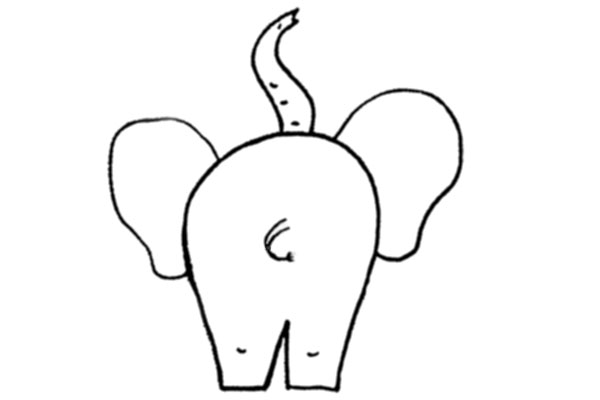
\includegraphics[scale=1.5]{images/slon.jpg}
\end{center}

\item
Укажите названия букв греческого алфавита и запишите соответствующие заглавные буквы:
\[\alpha, \zeta, \eta, \theta\].

\end{enumerate}



\newpage
\subsection[2014-2015]{\hyperref[sec:sol_kr_01_2014_2015]{2014-2015}}
\label{sec:kr_01_2014_2015}

\begin{enumerate}
\item Вася забыл какую-то (какую?) формулу. Он помнит, что она начинается
с «$\P(A|B) = $». Дальше была дробь, три буквы $\P$ со скобками после них и
в сумме по две буквы $A$ и $B$ внутри этих скобок. Ещё там была вертикальная черта «|».
Из этих элементов Вася случайным образом составляет формулу.
\begin{enumerate}
\item С какой вероятностью Вася напишет правильную формулу?
\item Напишите формулу, которую забыл Вася.
\end{enumerate}

Примечание: Вася всё-таки успел сходить на пару лекций по теории вероятностей и помнит,
что $\P(A|B)$ и $\P(B|A)$ — это не одно и то же, «|» должна стоять именно между буквами
(то ли $A|B$, то ли $B|A$), а в скобках, которые идут после $\P$, должно хоть что-то стоять.
При этом формула должна иметь смысл, то есть  $\P(A|B)$   не должна выражаться через себя же,
и дробь не должна быть сократимой.

\item Точка с координатами $(\xi, \eta)$ бросается наудачу в треугольник с вершинами
$(1,0)$, $(0,0)$, $(0,1)$. Сформулируйте определение независимости двух событий и
проверьте, будут ли события $A=\{ \xi < 1/2 \}$  и $B=\{ \eta < 1/2 \}$  независимыми?

\item На учениях три самолёта одновременно и независимо атакуют цель.
Известно, что первый самолёт поражает цель с вероятностью $0.6$, второй — $0.4$,
третий — $0.3$. При разборе учений выяснилось, что цель была поражена только
одним самолётом. Какова вероятность того, что это был первый самолёт?

\item Книга в $500$ страниц содержит $400$ опечаток. Предположим, что каждая
из них независимо от остальных опечаток может с одинаковой вероятностью оказаться
на любой странице книги.
\begin{enumerate}
\item Определите вероятность того, что на $13$-й странице будет не менее двух опечаток,
в явном виде и с помощью приближения Пуассона.
\item Определите наиболее вероятное число, математическое ожидание и дисперсию числа
опечаток на $13$-ой странице.
\item Является ли $13$-ая страница более «несчастливой», чем все остальные
(в том смысле, что на $13$-ой странице ожидается большее количество очепяток,
чем на любой другой)?
\end{enumerate}

Подсказка. Можно считать, что опечатки «выбирают» любую из страниц для своего
появления независимо друг от друга. Успех заключается в выборе $13$-ой страницы.
Вероятность успеха?

\item Вероятность того, что медицинский тест выявит наличие заболевания,
когда оно действительно есть, называется чувствительностью теста. Специфичностью
теста называется вероятность того, что тест покажет отсутствие заболевания,
когда пациент здоров. Вероятность того, что пациент болен, когда тест показал
наличие заболевания, называется прогностической силой теста. Предположим, что
только 1\,\%  всего населения страдает данным заболеванием.  Чувствительность
используемого теста равна $0.9$, а специфичность — $0.95$.
\begin{enumerate}
\item Какова вероятность того, что у случайно выбранного человека тест покажет
наличие заболевания?
\item Какова прогностическая сила теста? Что нужно сделать, чтобы её повысить?
\end{enumerate}

\item Функция плотности случайной величины $X$ имеет вид:
\begin{equation*}
f(x) =
 \begin{cases}
   1.5 (x-a)^2 &, x \in [0,a]\\
   1.5 (x+a)^2 &, x \in [-a,0]\\
   0 &, x \not\in [-a,a]
 \end{cases}
\end{equation*}

\begin{enumerate}
\item Найдите константу $a$, вероятность попадания в отрезок $\left[1/2, 2 \right]$,
математическое ожидание $X$ и дисперсию случайной величины $X$.
\item Нарисуйте функцию распределения случайной величины $X$.
\end{enumerate}

\item Вася случайным образом посещает лекции по ОВП (Очень Важному Предмету).
С вероятностью $0.9$ произвольно выбранная лекция полезна, и с вероятностью $0.7$ она интересна.
Полезность и интересность — независимые друг от друга и от номера лекции свойства.
Всего Вася прослушал 30 лекций.
\begin{enumerate}
\item Определите математическое ожидание и дисперсию числа полезных лекций и
числа интересных лекций, прослушанных Васей.
\item Определите математическое ожидание числа бесполезных и неинтересных лекций,
прослушанных Васей, и числа лекций, обладающих хотя бы одним из свойств (полезность,
интересность).
\end{enumerate}

\item Пусть $\E(X) = 1$, $\E(Y) = 2$, $\E\left(X^2\right) = 5$, $\E(XY) = -1$. Найдите:
\begin{enumerate}
\item $\E(2X + Y - 4)$
\item $\Var(X)$, $\Var(Y)$
\item $\Cov(X,Y)$, $\Corr(X,Y)$
\item $\Var(X-Y-1)$,  $\Var(X+Y+1)$
\item $\Cov(X-Y-1, X+Y+1)$,  $\Corr(X-Y-1, X+Y+1)$
\end{enumerate}

\item Совместное распределение случайных величин $X$ и $Y$ задано в виде таблицы:

\begin{center}
\begin{tabular}{ccc}
\toprule
 & $X=1$ & $X=2$ \\ \midrule
$Y=-1$ & $0.1$ & $0.2$ \\
$Y=0$ & $0.2$ & $0.3$ \\
$Y=1$ & $0$ & $0.2$ \\ \bottomrule
\end{tabular}
\end{center}

\begin{enumerate}
\item Найти частные распределения $Y$ и $Y^2$
\item Найти ковариацию случайных величин $X$ и $Y$
\item Можно ли утверждать, что случайные величины зависимы?
\end{enumerate}

\item Бонусная задача

Какова вероятность того, что наугад выбранный ответ на этот вопрос окажется верным
(искомую вероятность вычислить и записать!)?
\begin{enumerate}
\item 0.25
\item 0.5
\item 0.6
\item 0.25
\end{enumerate}
\end{enumerate}



\newpage
\subsection[2013-2014]{\hyperref[sec:sol_kr_01_2013_2014]{2013-2014}}
\label{sec:kr_01_2013_2014}


\begin{enumerate}
\item Вероятность застать Васю на лекции зависит от того, пришли ли на лекцию Маша и Алена.
Данная вероятность равна $0.18$, если девушек нет; $0.9$ — если обе девушки пришли на лекцию;
$0.54$ — если пришла только Маша и $0.36$ — если пришла только Алена.
Маша и Алена посещают лекции независимо друг от друга с вероятностями $0.4$ и $0.6$ соответственно.
\begin{enumerate}
\item Определите вероятность того, что на лекции присутствует Алена, если в аудитории есть Вася.
\item Кого чаще можно застать на тех лекциях, на которых присутствует Вася: Машу или Алену?
%\item При каком значении $p$ Вася посещает половину всех лекций?
\end{enumerate}

\item Страховая компания страхует туристов, выезжающих за границу,
от невыезда и наступления страхового медицинского случая за границей.
Застраховано 100 туристов. Вероятность «невыезда» за границу случайно
выбранного туриста — $0.002$, а страховые выплаты в этом случае — 2000 у.е.;
вероятность обращения за медицинской помощью за границей — $0.01$,
а страховые выплаты — 3000 у.е. Для каждого туриста рассмотрим две случайные
величины: $X_i$, равную 1 при невыезде за границу и 0 иначе, и $Y_i$, равную 1
при обращении за медицинской помощью и нулю иначе.
Обозначим $X=\sum_{i=1}^{100}X_i$ и $Y=\sum_{i=1}^{100}Y_i$.
\begin{enumerate}
\item Определите $\P(X=5)$, $\E(X)$, $\Var(X)$.
\item Наиболее вероятное число не выехавших туристов.
\item Вычислите математическое ожидание и дисперсию величины совокупных страховых выплат.
\end{enumerate}
Подсказка: Число обращений в страховую компанию для каждого туриста может быть
записано в виде $X_i+X_i Y_i$, так как медицинский страховой случай может наступить
только, если турист выехал за границу. Случайные величины $X_i$ и $Y_i$ независимы.

\item Функция плотности случайной величины $X$ имеет вид:
\begin{equation}
f(x)=\begin{cases}
ce^{-x}, \, x\geq 0 \\
ce^x, \, x<0
\end{cases}
\end{equation}
\begin{enumerate}
\item Найдите $c$, $\P(X \in [\ln 0.5,\ln 4])$, $\E(X)$, $\Var(X)$
\item Моменты всех порядков случайной величины $x$
\end{enumerate}

Подсказка: $\int_0^{\infty} x^n e^{-x} \, dx=n!$

\item Известно, что  $\E(X)=-1$, $\E(Y)=1$, $\Var(X)=9$, $\Var(Y)=4$, $\Corr(X,Y)=1$.
Найдите
\begin{enumerate}
\item $\E(Y-2X-3)$, $\Var(Y-2X-3)$
\item  $\Corr(Y-2X-3,X)$
\item Можно ли выразить $Y$ через $X$? Если да, то запишите уравнение связи.
\end{enumerate}

\item Совместное распределение доходов акций двух компаний $Y$ и $X$ задано в виде таблицы

\begin{center}
\begin{tabular}{@{}cccc@{}}
\toprule
    & $X=-1$ & $X=0$ & $X=1$ \\ \midrule
$Y=-1$ & $0.1$  & $0.2$   & $0.2$ \\
$Y=1$ & $0.2$  & $0.1$ & $0.2$ \\ \bottomrule
\end{tabular}
\end{center}

\begin{enumerate}
\item Найдите  частные распределения случайных величин $X$ и $Y$
\item Найдите $\Cov(X,Y)$
\item Можно ли утверждать, что случайные величины $X$ и $Y$ зависимы?
\item Найдите условное распределение случайной величины $X$ при условии $Y=-1$
\item Найдите условное математическое ожидание $\E(X\mid Y=-1)$
\end{enumerate}
\end{enumerate}



\newpage
\subsection[2012-2013]{\hyperref[sec:sol_kr_01_2012_2013]{2012-2013}}
\label{sec:kr_01_2012_2013}


\begin{enumerate}

\item Погода завтра может быть ясной с вероятностью $0.3$ и пасмурной с вероятностью $0.7$.
Вне зависимости от того, какая будет погода, Маша даёт верный прогноз с вероятностью $0.8$.
Вовочка, не разбираясь в погоде, делает свой прогноз по принципу: с вероятностью $0.9$
копирует Машин прогноз, и с вероятностью $0.1$ меняет его на противоположный.
\begin{enumerate}
\item Какова вероятность того, что Маша спрогнозирует ясный день?
\item Какова вероятность того, что Машин и Вовочкин прогнозы совпадут?
\item Какова вероятность того, что день будет ясный, если Маша спрогнозировала ясный?
\item Какова вероятность того, что день будет ясный, если Вовочка спрогнозировал ясный?
\end{enumerate}

\item Машин результат за контрольную, $M$, равномерно распределен на отрезке $[0;1]$.
Вовочка ничего не знает, поэтому списывает у Маши, да ещё может наделать ошибок при
списывании. Поэтому Вовочкин результат, $V$, распределен равномерно от нуля до Машиного
результата.
\begin{enumerate}
\item Найдите $\P(M>2V)$, $\P(M>V+0.1)$
\item Зачёт получают те, чей результат больше $0.4$. Какова вероятность того, что Вовочка получит зачёт? Какова вероятность того, что Вовочка получит зачёт, если Маша получила зачёт?
\end{enumerate}
Подсказка: попробуйте нарисовать нужные события в осях $(V,M)$

Это была задачка-неберучка!

\item Функция плотности случайной величины $X$ имеет вид
\[
f(x)=
\begin{cases}
\frac{3}{7}x^2, & x\in[1;2] \\
0,& x \notin [1,2]
\end{cases}
\]
\begin{enumerate}
\item Не производя вычислений найдите $\int_{-\infty}^{+\infty}f(x)\,dx$
\item Найдите $\E(X)$, $\E(X^2)$ и дисперсию $\Var(X)$
\item Найдите $\P(X>1.5)$
\item Найдите функцию распределения $F(x)$ и постройте её график
\end{enumerate}

\item Совместное распределение случайных величин $X$ и $Y$ задано таблицей

\begin{center}
\begin{tabular}{@{}cccc@{}}
\toprule
      & $X=-2$ & $X=0$ & $X=2$ \\ \midrule
$Y=1$ & $0.2$  & $0.3$ & $0.1$ \\
$Y=2$ & $0.1$  & $0.2$ & $a$   \\ \bottomrule
\end{tabular}
\end{center}

\begin{enumerate}
\item Определите неизвестную вероятность $a$.
\item Найдите вероятности $\P(X>-1)$, $\P(X>Y)$
\item Найдите математические ожидания $\E(X)$, $\E\left(X^2\right)$
\item Найдите корреляцию $\Corr(X,Y)$
\end{enumerate}

\item Винни Пух собрался полакомиться медом, но ему необходимо принять решение,
к каким пчелам отправиться за медом. Неправильные пчелы кусают каждого, кто лезет
к ним на дерево с вероятностью $0.9$, но их всего 10 штук. Правильные пчелы кусаются
с вероятностью $0.1$, но их 100 штук.
\begin{enumerate}
\item  Определите математическое ожидание и дисперсию числа укусов Винни Пуха для каждого случая
\item Определите наиболее вероятное число укусов и его вероятность для каждого случая
\item К каким пчелам следует отправиться Винни Пуху, если он не может выдержать больше двух укусов?
\end{enumerate}
\end{enumerate}



\section{Ответы}

\thispagestyle{empty}
\section{Ответы к минимумам}

\subsection[Кр 1]{\hyperref[sec:minimum_kr_01]{Контрольная работа 1 — Задачный минимум}}
\label{sec:sol_minimum_kr_01}



\begin{multicols}{2}
\begin{enumerate}
	\item
			\begin{enumerate}
				\item $0.25$
				\item $0.6$
				\item нет
			\end{enumerate}
	\item
			\begin{enumerate}
				\item $0.5$
				\item $0.75$
				\item нет
			\end{enumerate}
	\item $\frac{4}{10 \cdot 11 \cdot 12 \cdot 13}$
	\item $\frac{4}{10 \cdot 11 \cdot 12 \cdot 13}$
	\item $0.5$
	\item $0.42$
	\item $0.028$
	\item $\frac{5}{7}$
	\item
			\begin{enumerate}
				\item $0.5$
				\item $0.75$
				\item $0$
				\item $0.5$
			\end{enumerate}
	\item
			\begin{enumerate}
				\item $0.5$
				\item $0$
				\item $0.5$
				\item $0.5$
				\item $0.5$
			\end{enumerate}
	\item
			\begin{enumerate}
				\item $0.25$
				\item $0.75$
				\item $0$
				\item $0.5$
			\end{enumerate}
	\item
			\begin{enumerate}
				\item $0.25$
				\item $0.25$
				\item $0.75$
				\item $0.5$
				\item $0.75$
			\end{enumerate}
	\item
			\begin{enumerate}
				\item $\left( \frac{1}{4} \right) ^4$
				\item $1 - \left( \frac{1}{4} \right) ^4$
				\item $0$
				\item $3$
				\item $0.75$
				\item $2$, $3$
			\end{enumerate}
	\item
			\begin{enumerate}
				\item $\left( \frac{3}{5} \right) ^5$
				\item $1 - \left( \frac{3}{5} \right) ^5$
				\item $0$
				\item $2$
				\item $1.2$
				\item $2$
			\end{enumerate}
	\item
			\begin{enumerate}
				\item $e^{-100}$
				\item $1 - e^{-100}$
				\item $0$
				\item $100$
				\item $100$
			\end{enumerate}
	\item
			\begin{enumerate}
				\item $e^{-101}$
				\item $1 - e^{-101}$
				\item $0$
				\item $101$
				\item $101$
			\end{enumerate}
	\item $1 - \frac{8^5}{9^5}$
	\item $\frac{8^5}{9^5}$
	\item $1 - e^{-3}$
	\item $e^{-3}$
	\item
			\begin{enumerate}
				\item $0.5$
				\item $0.25$
				\item $0.125$
				\item $1$
			\end{enumerate}
	\item
			\begin{enumerate}
				\item $0.5$
				\item $0.5$
				\item $\frac{1}{3}$
				\item $\frac{1}{12}$
				\item $1$
			\end{enumerate}
	\item
			\begin{enumerate}
				\item $2$
				\item $0.25$
				\item $\frac{3}{4}$
				\item $1$
			\end{enumerate}
	\item
			\begin{enumerate}
				\item $2$
				\item $0.5$
				\item $0.5$
				\item $0$
				\item $0.8$
			\end{enumerate}
\end{enumerate}
\end{multicols}


\subsection[Кр 2]{\hyperref[sec:minimum_kr_02]{Контрольная работа 2 — Задачный минимум}}
\label{sec:sol_minimum_kr_02}


\begin{multicols}{2}
\begin{enumerate}

\item
\begin{enumerate}
\item   $0.5 $
\item   $0.3$
\item   $0.2$
\item   нет
\item   $0.3$
\item
\begin{tabular}{lrr}
\toprule
$x$ & $-1$  & $1$   \\ \midrule
$\P(X=x)$ & $0.5$ & $0.5$ \\ \bottomrule
\end{tabular}
\item  $F_{X}(x) = \begin{cases}
0, & \text{при } x < -1 \\
0.5 , & \text{при } x \in [-1;1) \\
1, & \text{при }  x \geq 1
\end{cases}$
\end{enumerate}
\item
\begin{enumerate}
\item   $0.5$
\item   $0.4$
\item   $0.2$
\item   да
\item   $0.6$
\item
\begin{tabular}{lrrr}
\toprule
$y$ & $-1$  & $0$   & $1$   \\ \midrule
$\P(Y=y)$ & $0.4$ & $0.2$ & $0.4$ \\ \bottomrule
\end{tabular}
\item   $F_{Y}(y) = \begin{cases}
0, & \text{при } y < -1 \\
0.4 , & \text{при } y \in [-1;0) \\
0.6, & \text{при }  y \in [0;1)\\
1, & \text{при } y \geq 1
\end{cases}$
\end{enumerate}

\item
\begin{enumerate}
\item $0$
\item $1$
\item $1$
\item $0$
\item $0.6$
\item $0.6$
\item $0$
\item $0$
\item $0$
\item да, являются некоррелированными, но нельзя утверждать, что являются независимыми
\end{enumerate}

\item
\begin{enumerate}
\item $0$
\item $1$
\item $1$
\item $0$
\item $0.8$
\item $0.8$
\item $0$
\item $0$
\item $0$
\item да, являются некоррелированными, но нельзя утверждать, что являются независимыми
\end{enumerate}

\item
\begin{enumerate}
\item $0.25$
\item $0.2$
\item Обозначим $A = \{X = -1\}$

\begin{tabular}{lrrr}
\toprule
$y$           & $-1$  & $0$   & $1$   \\ \midrule
$\P(Y=y|A)$   & $0.4$ & $0.2$ & $0.4$ \\ \bottomrule
\end{tabular}
\item $0$
\item $0.8 $
\end{enumerate}
\item
\begin{enumerate}
\item $0.5$
\item $0.2$
\item Обозначим $A = \{X = 1\}$
\begin{tabular}{lrrr}
\toprule
$y$ & $-1$  & $0$   & $1$   \\ \midrule
$\P(Y=y|A)$             & $0.4$ & $0.2$ & $0.4$ \\ \bottomrule
\end{tabular}
\item $0$
\item $0.8$
\end{enumerate}

\item
\begin{enumerate}
\item $0 $
\item $36$
\item $9 $
\item $60 $
\item $-4$
\item $\frac{-1}{3\sqrt{5}}$
\item $\begin{pmatrix}
 3 & -1 \\
-1 & 4
\end{pmatrix}$
\end{enumerate}

\item
\begin{enumerate}
\item $-4$
\item $8 $
\item $1 $
\item $10$
\item $-6$
\item$ \frac{-1}{\sqrt{5}}$

\item $\begin{pmatrix}
 1 & 1 \\
 1 & 2
\end{pmatrix}$
\end{enumerate}
\item
\begin{enumerate}
\item $0.3413$
\item $0.0228$
\item $0.1915$
\end{enumerate}

\item
\begin{enumerate}
\item $0.6826$
\item $0.0228$
\item $0.1574$
\end{enumerate}

\item $0.4332$
\item $0.8185$
\item $0.4514$
\item $0.5328$
\item $\approx 0.8185$
\item $\approx 0.9115$
\item $\approx 0.6422$
\item $\approx 0.9606$

\item
\begin{enumerate}
\item $0.125$
\item $0.5$
\item $f_{X}(x) = \begin{cases} x+\frac{1}{2}, & \text{при } x \in [0;1] \\ 0 , & \text{при } x \not\in [0;1] \end{cases}$
\item $f_{Y}(y) = \begin{cases} y+\frac{1}{2}, & \text{при } y \in [0;1] \\ 0 , & \text{при } y \not\in [0;1] \end{cases}$
\item нет
\end{enumerate}

\item
\begin{enumerate}
\item $\frac{1}{16}$
\item $\frac{1}{2}$
\item $f_{X}(x) =
\begin{cases} 2x, & \text{при } x \in [0;1] \\
0 , & \text{при } x \not\in [0;1]
\end{cases}$
\item $f_{Y}(y) =
\begin{cases} 2y, & \text{при } y \in [0;1] \\
0 , & \text{при } y \not\in [0;1]
\end{cases}$
\item да
\end{enumerate}
\item
\begin{enumerate}
\item $\frac{7}{12}$
\item $\frac{7}{12}$
\item $\frac{1}{3}$
\item $-\frac{1}{144}$
\item $-\frac{1}{11}$
\end{enumerate}

\item
\begin{enumerate}
\item $\frac{2}{3}$
\item $\frac{2}{3}$
\item $\frac{4}{9}$
\item $0$
\item $0$
\end{enumerate}

\item
\begin{enumerate}
\item $f_{Y}(y) =
\begin{cases} y+\frac{1}{2}, & \text{при } y \in [0;1] \\
0 , & \text{при } y \not\in [0;1]
\end{cases}$
\item $f_{X|Y}(x|\frac{1}{2}) =
\begin{cases} x+\frac{1}{2}, & \text{при } x \in [0;1] \\
0 , & \text{при } x \not\in [0;1]
\end{cases}$
\item $\frac{7}{12}$
\item $\frac{11}{144}$
\end{enumerate}

\item
\begin{enumerate}
\item $f_{Y}(y) =
\begin{cases} 2y, & \text{при } y \in [0;1] \\
0 , & \text{при } y \not\in [0;1]
\end{cases}$
\item $f_{X|Y}(x|\frac{1}{2}) =
\begin{cases} 2x, & \text{при } x \in [0;1] \\
0 , & \text{при } x \not\in [0;1]
\end{cases}$
\item $\frac{2}{3}$
\item $\frac{1}{18}$
\end{enumerate}
\end{enumerate}
\end{multicols}



\subsection[Кр 3]{\hyperref[sec:minimum_kr_03]{Контрольная работа 3 — Задачный минимум}}
\label{sec:sol_minimum_kr_03}


\begin{multicols}{2}
\begin{enumerate}
\item
\begin{enumerate}
\item $\approx 0.15$
\item $U \sim \cN(101,29)$, $f(u) = \frac{1}{\sqrt{2\pi\cdot 29}}e^{-\frac{1}{2}\frac{(u-101)^2}{29}}$
\item $\approx 0.02$
\end{enumerate}
\item
\begin{enumerate}
\item $71.14$
\item $f(y|x=170) = \frac{1}{\sqrt{2\pi\cdot20}}e^{-\frac{1}{2}\frac{(y-71.14)^2}{20}}$
\item $\approx 0$
\end{enumerate}
\item
\begin{enumerate}
\item $0.25$
\item $0.6875$
\item $0.91(6)$
\item $0.75$
\item $-0.28125$
\end{enumerate}
\item
\begin{enumerate}
\item $-1, 0, 1, 1$
\item $-1$
\item $1$
\item $f(x) = \begin{cases}
0, & x < -1 \\
0.25, & -1 \leq x < 0 \\
0.5, & 0 \leq x < 1 \\
1, & x \geq 1
\end{cases}$
\end{enumerate}
\item
\begin{enumerate}
\item $\theta$
\item да
\end{enumerate}

\item
\begin{enumerate}
\item нет, оценка смещена
\item $c = 2$
\end{enumerate}
\item
\begin{enumerate}
\item все оценки несмещенные
\item $\hat{p}_3$ наиболее эффективная
\end{enumerate}
\item да
\item да
\item $\hat{\theta}_{MM} = \sqrt{\frac{\sum_{i=1}^n(X_i-\overline{X})^2\cdot20}{n}}$

\item $\hat{\theta}_{MM} = \frac{1}{5}\left(6 - \frac{1}{n}\sum_{i=1}^n X_i^2 \right)$, $\hat{\theta}_{MM} = 0.68$
\item $\hat{\theta}_{ML} = \frac{\sum_{i=1}^n x_i^2}{n}$
\item $\hat{p}_{ML} = \frac{\sum_{i=1}^n x_i}{n}$
\item да
\item $n_1 \approx 260$, $n_2 \approx 232$, $n_3 \approx 658$

\end{enumerate}
\end{multicols}






\subsection[Кр 4]{\hyperref[sec:minimum_kr_04]{Контрольная работа 4 — Задачный минимум}}
\label{sec:sol_minimum_kr_04}


\begin{enumerate}
\item $\left[-1.6 - 1.65 \cdot \frac{2}{\sqrt{3}}; -1.6 + 1.65 \cdot \frac{2}{\sqrt{3}} \right]$
\item $\left[-1.6 - 2.92 \cdot \sqrt{\frac{18.33}{3}}; -1.6 + 2.92 \cdot \sqrt{\frac{18.33}{3}} \right]$
\item $\left[\frac{17.43 \cdot 2}{4.61}; \frac{17.43 \cdot 2}{0.21} \right]$
\item $\left[-1.6 - (-2.6) - 1.96 \cdot \sqrt{\frac{2}{3} + \frac{1}{2}}; -1.6 - (-2.6) + 1.96 \cdot \sqrt{\frac{2}{3} + \frac{1}{2}} \right]$
\item $\left[1.04 - (-0.37) - 3.18 \cdot \sqrt{3.02} \sqrt{\frac{1}{3} + \frac{1}{2}}; 1.04 - (-0.37) + 3.18 \cdot \sqrt{3.02} \sqrt{\frac{1}{3} + \frac{1}{2}} \right]$
\item $\left[0.45 - 1.96 \cdot \sqrt{\frac{0.45 \cdot 0.55}{100}}; 0.45 + 1.96 \cdot \sqrt{\frac{0.45 \cdot 0.55}{100}} \right]$
\item $\left[0.6 - 0.4 - 1.96  \cdot \sqrt{\frac{0.6\cdot0.4}{100} + \frac{0.4 \cdot 0.6}{200}}; 0.6 - 0.4 + 1.96 \cdot \sqrt{\frac{0.6\cdot0.4}{100} + \frac{0.4 \cdot 0.6}{200}} \right]$
\item $\left[2.5 - 1.96 \cdot \sqrt{\frac{1}{40}}; 2.5 + 1.96 \cdot \sqrt{\frac{1}{40}} \right]$
\item $\left[\frac{1}{0.52} - 1.96 \cdot \sqrt{\frac{1}{100 \cdot 0.52^2}}; \frac{1}{0.52} + 1.96 \cdot \sqrt{\frac{1}{100 \cdot 0.52^2}} \right]$
\item
\begin{enumerate}
\item $\approx 0.02$
\item $\approx 0.02$
\item $\approx 0.98$
\end{enumerate}
\item $0.2$
\item $z_{obs} \approx -1.39 $, $z_{crit} = 1.28$, нет оснований отвергать $H_0$.
\item $t_{obs} \approx -0.65$, $t_{crit} = 1.89$, нет оснований отвергать $H_0$.
\item $z_{obs} \approx 0.93$, $z_{crit} = -1.65$, нет оснований отвергать $H_0$.
\item $t_{obs} \approx 0.89$, $t_{crit} = -2.35$, нет оснований отвергать $H_0$.
\item $F_{obs} \approx 95.37$, $F_{crit} = 199.5$, нет оснований отвергать $H_0$.
\item $z_{obs} \approx 2.04$, $z_{crit} = 1.65$, основная гипотеза отвергается.
\item $z_{obs} \approx 4.16$, $z_{crit} = 1.96$, основная гипотеза отвергается.
\item $\gamma_{obs} \approx 0.26$, $\gamma_{crit} = 5.99$, нет оснований отвергать $H_0$.
\item $\gamma_{obs} \approx 139.4$, $\gamma_{crit} = 3.84$, основная гипотеза отвергается.
\item $LR_{obs} \approx 5.5$, $LR_{crit} = 3.84$, основная гипотеза отвергается.
\end{enumerate}

\subsection*{Решения контрольной номер 1}

\subsubsection*{\hyperref[sec:kr_01_2017_2018]{2017-2018}}
\label{sec:sol_kr_01_2017_2018}

\begin{enumerate}
\item
\begin{enumerate}
\item События называются независимыми, если  $ \P(A \cap B) = \P(A) \cdot \P(B)$
\item Запасёмся всеми нужными вероятностями:

$\P(A) = \frac{1}{2}$

$\P(B) = \frac{1}{3}$

$\P(C) = \frac{1}{2}$

$\P(A \cap C) = \frac{1}{3} $ — выпадет чётое число больше трёх

$\P(A \cap B)  = \frac{1}{6}$ — выпадет чётное число, кратное трём

$\P(A \cap C) = \frac{1}{6}$ — выпадет число, большее трёх и кратное трём

Теперь можно проверять независимость:

$\P(A \cap C) \neq \P(A) \cdot \P(C) \Rightarrow$  не являются независимыми

$ \P(A \cap B) = \P(A) \cdot \P(B) \Rightarrow$ являются независимыми

$ \P(B \cap C) = \P(B) \cdot \P(C) \Rightarrow$ являются независимыми

\end{enumerate}
\item
\begin{enumerate}
\item Количество возможных вариантов ТМ: $ C_{10}^2 $,  количество возможных вариантов ЗМ: $ C_{24}^2 $. Количество их возможных сочетаний: $ C_{10}^2 \cdot C_{24}^2$ , где $ C_n^k = \frac{n!}{k!(n-k)!}$.
\item По классическому определению вероятностей, предполагая исходы равновероятными, искомая вероятность равна $ \frac{C_{16}^2}{C_{24}^2} $
\item По тому же принципу:
\[
\frac{C_k^2}{C_{10}^2} = \frac{1}{15} \Rightarrow \frac{\frac{k!}{2!(k-2)!}}{\frac{10!}{2! \cdot 8!}} = \frac{1}{15} \Rightarrow \frac{(k-1)k}{2}\frac{ 2}{9 \cdot 10} = \frac{1}{15}
\]
Получаем квадратное уравнение вида $ k^2 - k - 6 = 0 $ с корнями $-2$ и $3$. Так как $k$ не может быть отрицательным, ответ $3$.
\end{enumerate}
\item
\begin{enumerate}
\item Если эксперт отдаёт предпочтение Fit, то это можно интерпретировать как «успех» в схеме Бернулли. Так как $\xi$ - количество успехов, $ k \in [0;4]$, $p = \frac{1}{3} $, то
\[
\P(\xi = k) = C_n^k(p)^k(1-p)^{n-k}
\]

Большинство означает, что либо три, либо четыре эксперта выбрали Fit.
\[
\P(\xi = 3) = C_4^3\left(\frac{1}{3}\right)^3 \left(\frac{2}{3}\right)^{1} = \frac{8}{81}
\]
\[
\P(\xi = 4) = C_4^4\left(\frac{1}{3}\right)^4 \left(\frac{2}{3}\right)^{0} = \frac{1}{81}
\]
\[
\P( \xi > 2) =  \frac{9}{81}
\]
\item Аналогично:

\[ \P(\xi = 0) = C_4^0\left(\frac{1}{3}\right)^0 \left(\frac{2}{3}\right)^{4} = \frac{16}{81}\]

\[ \P(\xi = 1) = C_4^1\left(\frac{1}{3}\right)^1 \left(\frac{2}{3}\right)^{3} = \frac{32}{81}\]

\[ \P(\xi = 2) = C_4^2\left(\frac{1}{3}\right)^2 \left(\frac{2}{3}\right)^{2} = \frac{24}{81}\]

\begin{figure}[h!]
    \noindent\centering{
    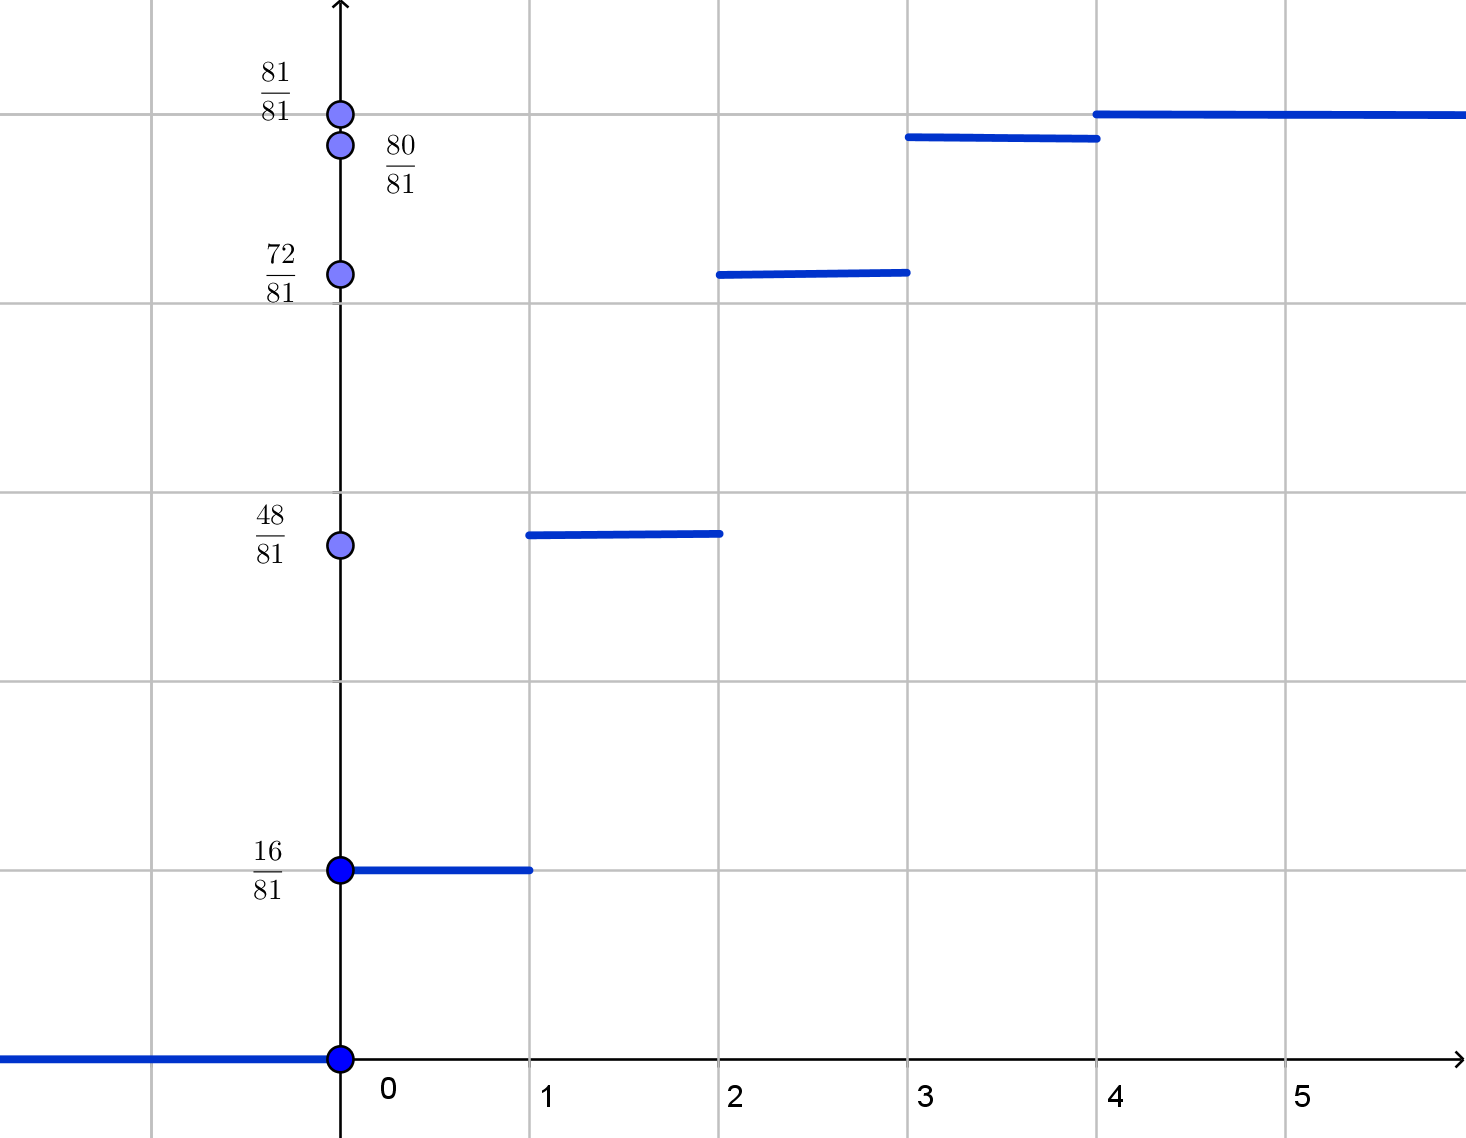
\includegraphics[width=80mm]{images/kr1_2017_3.png}
    }
    \caption{Функция распределения}
    \label{cdf_kr2017}
\end{figure}

\item Все вероятности посчитаны, видим, что наибольшая достигается при $\xi=1$.
\item $\E(X) = np = \frac{4}{3} $, $ \Var(X) = npq = \frac{8}{9}$
\end{enumerate}
\item
\begin{enumerate}
\item Так как указано, что цена сметаны распределена равномерно на отерзке $[250, 1000]$, максимальное значение цены — $1000$, это и есть необходимая сумма.
\item Вспомним, что функция распределения $F(x) = \P(X \leq x)$, нужно найти такой $x$, что $ \P(X \leq x)=0.9$:
\[
0.9 = 1 - \exp({-x^{2}}) \Rightarrow \exp(-x^{2}) = 0.1 \Rightarrow -x^2 = \ln(0.1)  \Rightarrow x=  \sqrt{-\ln(0.1)}
\]
\item Взяв производную от функции распределения списка без сметаны, получим функцию плотности:
\[
f_X(x) =
\begin{cases}
2x\exp(-x^2) & x \ge 0 \\
0 & \text{иначе}
\end{cases}
\]
Найдём математическое ожидание:
\[
\int_{0}^{+\infty}2x^2\exp({-x^2}) dx = -x \exp({-x^2})\big|_0^{+\infty} + \int_{0}^{+\infty}\exp({-x^2}) dx = \frac{\sqrt{\pi}}{2}
\]
\item Математическое ожидание суммы случайных величин равно сумме математических ожиданий случайных влечин, если они существуют. Математическое ожидание от цены сметаны равно: $ \frac{1000 + 250}{2} = 625 $
Математическое ожидание списка без сметаны было найдено в предыдущем пункте, его осталось перевести в рубли. Получаем ответ: $ 625 + \frac{\sqrt{\pi}}{2} \cdot 1000 $.
\item Так как обе величины имеют абсолютно непрерывные распределения, вероятность попасть в конкретную точку равна нулю.
\end{enumerate}
\item
\begin{enumerate}
\item $\P(\text{детектор показал ложь и подозреваемый лжёт}) = 0.9 \cdot 0.1 + 0.1 \cdot 0.95 = 0.185$
\item $\P(\text{невиновен}|\text{детектор показал ложь}) = \frac{0.9\cdot0.1}{0.185} = \frac{90}{185}$
\item $\P(\text{эксперт точно выявит преступника}) = (0.9)^9 \cdot 0.95$
\item $\P(\text{эксперт ошибочно выявит преступника}) = 9 \cdot 0.1 \cdot 0.9^8\cdot 0.05$
\end{enumerate}
\end{enumerate}


\subsubsection*{\hyperref[sec:kr_01_2016_2017]{2016-2017}}
\label{sec:sol_kr_01_2016_2017}

\begin{enumerate}
\item
\begin{enumerate}
\item Возможны четыре равновероятные ситуации:
\[
\P(\text{ММ}) = \P(\text{МД}) = \P(\text{ДМ}) = \P(\text{ДД}) = 1/4
\]

Посчитаем условную вероятность:
\[
\P(B \mid A) = \frac{\P(B \cap A)}{\P(A)} = \frac{\P(\text{МД, ДМ})}{\P(\text{ДМ, МД, ДД})} = \frac{2/4}{3/4} = \frac{2}{3}
\]

\item События $A$ и $B$ называются независимыми, если $\P(A \cap B) = \P(A) \cdot \P(B)$

В нашем случае: $\P(A \cap B) = \P (\text{МД, ДМ}) = 2/4$,
$\P(A) \cdot \P (B) = 3/4 \cdot 3/4$.

Следовательно, $\P(A \cap B) \neq \P(A) \cdot \P (B)$,
значит, события $A$ и $B$ не являются независимыми.
\end{enumerate}

\item Пусть событие $A_i$ означает, что $i$-ый узел системы дал сбой,
а событие $B_N$, что вся система дала сбой.

В условии сказано, что $\P(A_i) = 10^{-6}$,
а найти нужно такое максимальное $N \in \mathbb{N}$, при котором

\[
\P(B_N) \leq \frac{1}{10^2}
\]

\begin{align*}
\P(B_N) &= \P\left(\cup_{i=1}^n A_i\right) = 1 - \P (\left(\cup_{i=1}^n A_i\right)^c) \\
&\stackrel{\text{ф-ла де Моргана}}{=} 1 - \P \left(\cup_{i=1}^N A_i^c\right) \stackrel{A_1, \ldots, A_N \text{– независ.}}{=} 1 - \P(A_1^c) \cdot \ldots \cdot \P(A_N^c) \\
&= 1 - \left(1-\frac{1}{10^6}\right)^N
\end{align*}
Чтобы найти такое максимальное $N \in \mathbb{N}$, надо решить следующее неравенство
\begin{align*}
& 1 - \left(1-10^{-6}\right)^N \leq 10^{-2} \\
& 1 - 10^{-2} \leq \left(1-10^{-6}\right)^N \\
& \ln\left(1 - 10^{-2}\right) \leq N \ln \left(1 - 10^{-6}\right) \\
& N \leq \frac{\ln\left(1 - 10^{-2}\right)}{ \ln \left(1 - 10^{-6}\right)} \approx 10050.33
\end{align*}
Значит, максимальное $N$ равно $10050$.

\item Введём обозначения для событий.
Пусть $A$ означает, что человек имеет заболевание лёгких,
а $B$, что человек работал в шахте.

В условии сказано, что $\P(B \mid A) = 0.22$, $\P(B \mid A^c) = 0.14$, $\P(A) = 0.04$.
\begin{enumerate}
\item Нужно найти
\[
\P(A \mid B) = \frac{\P(A\cap B)}{\P (B)} = \frac{\P(B|A)\P(A)}{\P(B)}
\]
Для этого с помощью формулы полной вероятности посчитаем
\[
\P (B) = \P (B \mid A) \P(A) + \P (B \mid A^c) \P (A^c) = 0.22 \cdot 0.04 + 0.14 \cdot 0.96 = 0.1432
\]
Осталось подставить значения:
\[
\P(A \mid B) = \frac{0.22 \cdot 0.04}{0.1432} \approx 0.0615
\]

\item Все необходимые значения для второго пункта у нас есть,
осталось применить формулу условной вероятности:
\begin{multline*}
\P  (A \mid B^c) =  \frac{\P(A\cap B^c)}{\P (B^c)} =  \frac{\P (B^c \cap A)}{\P(A)} \cdot \frac{\P(A)}{\P (B^c)} = \P (B^c \mid A) \cdot \frac{\P(A)}{\P (B^c)} = \\
= (1-\P (B \mid A)) \cdot \frac{\P(A)}{1-\P (B)} = (1-0.22) \cdot \frac{0.04}{1-0.1432} \approx 0.0364
\end{multline*}
\end{enumerate}
\item Введём индикатор события «Петя дал верный ответ на $i$-ый вопрос»:
\[
X_i =
\begin{cases}
1, & \text{если на } i \text{-ый вопрос теста Петя дал верный ответ} \\
0, & \text{иначе}
\end{cases}
\]

Заметим, что $X_i \sim Be\left(p = 1/5 \right)$, $X_1, \ldots, X_{17}$ – независимы,
$X = X_1 + \ldots + X_{17}$ – общее число верных ответов,
$X \sim Bin\left(n=17, p=1/5\right)$.

\begin{enumerate}
\item Наибольшее вероятное число правильных ответов $m_0$ может быть нвйдено по формуле:
\begin{enumerate}
\item[1)] если число $(n\cdot p - q)$ – не целое, где $q:=1-p$, то
\[
m_0 = [np-q] +1,
\]
\item[2)] если число  $(n\cdot p - q)$ – целое, то наиболее вероятных значений $m_0$ два:
\[
m_0' = np-q \text{ и } m_0'' = np-q+1
\]
\end{enumerate}
Итак, поскольку $np-q = 17\cdot\frac{1}{5} - \frac{4}{5} = 2.6$ – не целое, наиболее вероятное число верных ответов $m_0$ может быть найдено по формуле из пункта (1):
\[
m_0 = [np-q] +1 = [2.6] + 1 = 3
\]
\item \[\E(X) = np = 17 \cdot \frac{1}{5}=3.4\]

\[\Var(X) = npq = 17 \cdot \frac{1}{5} \cdot \frac{4}{5} = 2.72\]

\item
\begin{multline*}
\P (\text{Петя получит «отлично»}) = \P (X\geq 15) = \P (X = 15) + \P (X= 16) + \\
+ \P (X = 17) = C^{15}_{17} \cdot \left(\frac{1}{5}\right)^{15} \cdot \left(\frac{4}{5}\right)^2 + C^{16}_{17} \cdot \left(\frac{1}{5}\right)^{16} \cdot \left(\frac{4}{5}\right)^1 + C^{17}_{17} \cdot \left(\frac{1}{5}\right)^{17} \cdot \left(\frac{4}{5}\right)^0 = \\
= 136 \cdot \frac{16}{5^{17}} + 17 \cdot \frac{4}{5^{17}} + \frac{1}{5^{17}} \approx 2.94 \cdot 10^{-9}
\end{multline*}
\item Рассмотрим первый вопрос теста. Петя может выбрать первый ответ с вероятностью $1/5$, и Вася
может выбрать первый ответ с вероятностью $1/5$. Тогда они оба выберут одинаковый ответ с вероятностью $1/25$.
Вариантов ответа в каждом вопросе $5$, значит, вероятность совпадения ответа в одном вопросе равна $1/5$.
Всего вопросов 17, тогда получаем
\[
\P(\text{все ответы Пети и Васи совпадают}) = \left(\frac{1}{5}\right)^{17}
\]

\end{enumerate}
\item Введём случайную велчину $\eta$, которая означает число потенциальных покупателей, с которыми контактировал продавец оборудования. По условию задачи, $\eta$ имеет таблицу распеределения:
\begin{center}
\begin{tabular}{ccc}
\toprule
$\eta$ & $ 1 $ & $2$ \\ \midrule
$\P_{\eta}$ & $1/3$ & $2/3$ \\ \bottomrule
\end{tabular}
\end{center}
Случайная величина $\xi$ может принимать значения $0, 50000$ и $100000$
\begin{enumerate}

\item Найдём $\P (\xi = 0 )$. По формуле полной вероятности, имеем:
\begin{multline*}
\P (\xi = 0) = \P (\xi = 0 \mid \eta = 1 ) \cdot \P ( \eta = 1 ) + \P (\xi = 0 \mid \eta = 2 )  \cdot \P ( \eta = 2 )  = \\
= 0.9 \cdot \frac{1}{3} + 0.9\cdot0.9 \cdot \frac{2}{3} = 0.84
\end{multline*}

\item Найдём $\P (\xi = 50000 )$ и $\P (\xi = 100000 )$ :
\begin{multline*}
\P (\xi = 50000 ) =  \P (\xi = 50000 \mid \eta = 1 ) \cdot \P ( \eta = 1  ) +  \P (\xi = 50000 \mid \eta = 2 ) \cdot  \P ( \eta = 2 )  = \\
= 0.1 \cdot \frac{1}{3} + 2 \cdot 0.1 \cdot 0.9 \cdot \frac{2}{3} = 0.15(3)
\end{multline*}
\begin{multline*}
\P (\xi = 100000 ) =  \P (\xi = 100000 \mid \eta = 1 ) \cdot \P ( \eta = 1 ) +  \P (\xi = 100000 \mid \eta = 2 ) \cdot  \P ( \eta = 2  )  =  \\
= 0 \cdot \frac{1}{3} + 0.1\cdot 0.1  \cdot \frac{2}{3} = 0.00(6)
\end{multline*}
Таблица распределения случайной величина $\xi$ имеет вид:

\begin{center}
\begin{tabular}{cccc}
\toprule
$\xi$ & $ 0 $ & $5000$ & $100000$ \\ \midrule
$\P_{\xi}$ & $0.84$ & $0.15(3)$ & $0.00(6)$ \\ \bottomrule
\end{tabular}
\end{center}

Тогда функция распределения случайной величины $\xi$ имеет вид:
\[
F_{\xi} (X) =
\begin{cases}
0 & \text{при } x<0 \\
0.84 & \text{при } 0 \leq x < 50000 \\
0.84 + 0.15(3) & \text{при } 50000
\leq x < 100000 \\
1 & \text{при } x > 100000
\end{cases}
\]
Опр.: $F_{\xi} = \P (\xi \leq x ), x \in \mathbb{R}$
\item \[\E (X) = 0 \cdot 0.84 + 50000 \cdot 0.15(3) + 100000 \cdot 0.00(6) = 8333.(3)	\]
\begin{multline*}
\Var(X) = (0 - 8333.(3))^2 \cdot 0.84 + (50000-8333.(3))^2 \cdot 0.15(3) + \\
+ (100000 - 8333.(3))^2 \cdot 0.00(6) = 380555555.(5)
\end{multline*}
\end{enumerate}
\item
\begin{enumerate}
\item $ f_{\xi} (x)=
\begin{cases}
\frac{1}{b} & \text{при } x \in [0, b] \\
0 & \text{при } x \notin [0, b]
\end{cases}
$
\item  Известно, что если $\xi \sim U[a, b]$, то $\E (\xi) = \frac{a+b}{2}$. Стало быть, из уравнения $\E (\xi) = 1$ получаем $\frac{b}{2} = 1$,  то есть $b=2$.
\item Известно, что если $\xi \sim U[a, b]$, то $\Var (\xi) = \frac{(b-a)^2}{12}$. Значит, $\Var (\xi) = \frac{2^2}{12} = \frac{1}{3}$
\item Воспользуемся формулой $\P (\xi \in B ) = \int_B f_{\xi} (x) dx$. Имеем:
\[
\P (\xi > 1 ) = \P (\xi \in (1, + \infty) ) = \int_{1}^{+ \infty} f_{\xi} (x) dx = \int_{1}^{2} \frac{1}{2} dx = \frac{1}{2}
\]
\item Требуется найти такое минимальное число $q_{0.25}$, что $\int_{-\infty}^{q_{0.25}} f_{\xi} (x) dx = 0.25$. Итак:
\[
\int_{-\infty}^{q_{0.25}} f_{\xi} (x) dx = 0.25 \Leftrightarrow \int_{-\infty}^{q_{0.25}} \frac{1}{2} dx = 0.25 \Leftrightarrow \frac{1/2}{q_{0.25}} = 0.25 \Leftrightarrow
\]
\[
q_{0.25} = 2 \cdot 0.25 = 0.5
\]
\item
\begin{multline*}
\E [ (\xi - \E(\xi))^{2017} ] = \int_{-\infty}^{+\infty} (x- \E(\xi) )^{2017} \cdot f_{\xi} (x) dx = \int_{-\infty}^{+\infty} (x-1)^{2017} f_{\xi} (x) dx = \\
= \int_{0}^{2} (x-1)^{2017} \cdot \frac{1}{2} dx = \frac{(x-1)^{2018}}{2018} \cdot \frac{1}{2} \bigg\rvert_{x=0}^{x=2} =0
\end{multline*}
\item $F_{\xi} (x) =
\begin{cases}
0 & \text{при } x < 0 \\
\frac{x}{2} & \text{при } 0 \leq x \leq 2 \\
1 & \text{при } x > 2
\end{cases}
$
\item Согласно условиям задачи, время до прихода 1-го поезда есть $\xi$; время до прихода 2-го поезда равно $\xi + b$; время до прихода 3-го (заветного) поезда есть $\xi + 2b$. Таким образом, Марья Ивановна в среднем ожидает «своего» поезда $\E (\xi + 2b) = 1 + 2b = 1 + 2 \cdot 2 = 5 $ минут. При этом $\Var (\xi + 2b) = \Var (\xi) = 1/3$
\item[к)] Пусть $\tau$ – наименьший номер поезда без «подозрительных лиц». По условию задачи, таблица распределения случайной величины $\tau$ имеет вид:

\begin{center}
\begin{tabular}{cccccc}
\toprule
$\tau$ & $ 1 $ & $2$ & $3$ & $4$ & \ldots \\ \midrule
$\P_{\tau}$ & $1/4$ & $3/4\cdot1/4$ & $(3/4)^2 \cdot 1/4$ & $(3/4)^3 \cdot 1/4$ & \ldots\\ \bottomrule
\end{tabular}
\end{center}

То есть случайная величина $\tau$ имеет геометрическое распределение с параметром $p=1/4$ $(\tau \sim G(p=1/4))$.

Несложно сообразить, что время ожидания Глафирой Петровной «своего» поезда составляет: $\eta := \xi + b(\tau- 1)$. Стало быть, $\E (\eta) = \E (\xi) + b \cdot (\E(\tau)-1)  = 1 + 2 \cdot (4-1) = 7$ минут.

Здесь мы воспользовались тем фактом, что если $\eta \sim G(p)$, то $\E (\eta) = 1/p$
\item[и)] Найдём теперь вероятность $\P (\eta \geq 5 )$. Для нахождения искомой вероятности воспользуемся формулой полной вероятности:
\[
	\P (\eta \geq 5 ) = \P(\eta \geq 5, \tau < 3) +\P(\eta \geq 5, \tau = 3)+\P(\eta \geq 5, \tau > 3)
\]

Если Глафира уехала на первом или втором поезде,
то ждать больше 5 минут она не могла, то есть $\P(\eta \geq 5, \tau <3)=0$.

Если Глафира уехала на третьем поезде, то чтобы ждать больше пяти минут,
ей нужно ждать первый поезд больше минуты,
то есть $\P(\eta \geq 5, \tau = 3)=0.5 \P(\tau = 3)$.

Если Глафира уехала на четвертом поезде или позже, то она точно ждала больше 5 минут,
$\P(\eta \geq 5, \tau >3)=\P(\tau>3)$.

\[
\P(\eta \geq 5) = 0.5\P(\tau = 3) + \P(\tau > 3) = 0.5 \cdot (3/4)^2 \cdot (1/4) + (3/4)^3 = 63 / 128
\]

\end{enumerate}
\item Пусть $\xi$ — случайная величина, обозначающая число остановок лифта. Предствим её в виде суммы $\xi = \xi_2 + \ldots + \xi_{10}$, где $\xi_i$ — индикатор
того, что лифт остановился на $i$-ом этаже, то есть
\[
\xi_i = \begin{cases}
1 & \text{если лифт остановился} \\
0 & \text{иначе}
\end{cases}
\quad \forall i = 2, \ldots, 10
\]
Найдём соответсвующие вероятности:
\[
\P(\xi_i = 0) = \left(\frac{8}{9}\right)^9
\]
\[
\P(\xi_i = 1) = 1 - \P(\xi = 0) = 1 - \left(\frac{8}{9}\right)^9
\]
Тогда $\E(\xi_i) = \P(\xi_i = 0) \cdot 0 + \P(\xi_i = 1) \cdot 1 = 1 - \left(\frac{8}{9}\right)^9$, и в итоге получаем:
\[
\E(\xi) = 9 \cdot \E(\xi_i) = 9 \cdot \left(1 - \left(\frac{8}{9}\right)^9\right)
\]
\end{enumerate}

\subsubsection*{\hyperref[sec:kr_01_2015_2016]{2015-2016}}
\label{sec:sol_kr_01_2015_2016}

\begin{enumerate}
\item
\begin{enumerate}
\item[$\alpha$)] Найдём вероятности каждого события:
$\P(A) = 1/2$, $\P(B) = 1/2$, $\P(C) = 1/2$.

Проверим попарную независимость:
\begin{itemize}
\item $\P(A \cap B) = 1/4$, $\P(A) \cdot \P(B) = 1/2 \cdot 1/2 = 1/4$
\item $\P(A \cap C) = 1/4$, $\P(A) \cdot \P(C) = 1/2 \cdot 1/2 = 1/4$
\item $\P(B \cap C) = 1/4$, $\P(B) \cdot \P(C) = 1/2 \cdot 1/2 = 1/4$
\end{itemize}
Значит, события попарно независимы.
\item[$\beta$)] События $A_1, A_2, A_3$ называются независимыми в совокупности,
если $\P(A_1 \cap A_2 \cap A_3) = \P(A_1) \cdot \P(A_2) \cdot \P(A_3)$.

В нашем случае: $\P(A \cap B \cap C) = 0$, $ \P(A) \cdot \P(B) \cdot \P(C) = (1/2)^3$,
следовательно, события не являются независимыми в совокупности.
\end{enumerate}

\item
\begin{enumerate}
\item[$\alpha$)] Воспользуемся формулой полной вероятности:
\begin{align*}
\P(\text{выпала «6»}) &= \P(\text{выпала «6»} \mid \text{взят белый кубик}) \cdot \P(\text{взят белый кубик}) \\
&+ \P(\text{выпала «6»} \mid \text{взят красный кубик}) \cdot \P(\text{взят красный кубик}) \\
&= \frac{1}{6} \cdot \frac{1}{2} + \frac{1}{3} \cdot \frac{1}{2} = \frac{1}{4}
\end{align*}
\item[$\beta$)] Воспользуемся формулой условной вероятности и результатом предыдущего пункта:
\begin{align*}
\P(\text{взят красный кубик} \mid \text{выпала «6»}) &= \frac{\P(\text{взят красный кубик} \cap \text{выпала «6»})}{\P(\text{выпала «6»})}  \\
&= \frac{\frac{1}{2}\cdot \frac{1}{3}}{\frac{1}{4}} = \frac{2}{3}
\end{align*}
\end{enumerate}

\item
\begin{enumerate}
\item[$\alpha$)] Совместное распределение имеет вид:
\begin{center}
\begin{tabular}{@{}lllllll@{}}
\toprule
$\eta$ $\backslash$ $\xi$ & $1$                            & $2$                            & $3$                            & $4$                            & $5$                            & $6$                            \\ \midrule
$1$           & $\frac{2}{15}\cdot\frac{1}{6}$ & $\frac{2}{15}\cdot\frac{1}{6}\mbox{*}$  & $\frac{2}{15}\cdot\frac{1}{6}\mbox{*}$   & $\frac{2}{15}\cdot\frac{1}{6} \mbox{*}$   & $\frac{2}{15}\cdot\frac{1}{6} \mbox{*}$   & $\frac{1}{3}\cdot\frac{1}{6} \mbox{*}$   \\
$2$           & $\frac{2}{15}\cdot\frac{1}{6}$ & $\frac{2}{15}\cdot\frac{1}{6}$ & $\frac{2}{15}\cdot\frac{1}{6}\mbox{*}$   & $\frac{2}{15}\cdot\frac{1}{6}\mbox{*}$   & $\frac{2}{15}\cdot\frac{1}{6}\mbox{*}$   & $\frac{1}{3}\cdot\frac{1}{6} \mbox{*}$   \\
$3$           & $\frac{2}{15}\cdot\frac{1}{6}$ & $\frac{2}{15}\cdot\frac{1}{6}$ & $\frac{2}{15}\cdot\frac{1}{6}$ & $\frac{2}{15}\cdot\frac{1}{6} \mbox{*}$   & $\frac{2}{15}\cdot\frac{1}{6} \mbox{*}$   & $\frac{1}{3}\cdot\frac{1}{6} \mbox{*}$   \\
$4$           & $\frac{2}{15}\cdot\frac{1}{6}$ & $\frac{2}{15}\cdot\frac{1}{6}$ & $\frac{2}{15}\cdot\frac{1}{6}$ & $\frac{2}{15}\cdot\frac{1}{6}$ & $\frac{2}{15}\cdot\frac{1}{6} \mbox{*}$ & $\frac{1}{3}\cdot\frac{1}{6} \mbox{*}$   \\
$5$           & $\frac{2}{15}\cdot\frac{1}{6}$ & $\frac{2}{15}\cdot\frac{1}{6}$ & $\frac{2}{15}\cdot\frac{1}{6}$ & $\frac{2}{15}\cdot\frac{1}{6}$ & $\frac{2}{15}\cdot\frac{1}{6}$ & $\frac{1}{3}\cdot\frac{1}{6} \mbox{*}$   \\
$6$           & $\frac{2}{15}\cdot\frac{1}{6}$ & $\frac{2}{15}\cdot\frac{1}{6}$ & $\frac{2}{15}\cdot\frac{1}{6}$ & $\frac{2}{15}\cdot\frac{1}{6}$ & $\frac{2}{15}\cdot\frac{1}{6}$ & $\frac{1}{3}\cdot\frac{1}{6}$ \\ \bottomrule
\end{tabular}
\end{center}
\item[$\beta$)] $\P(\text{выиграет белый кубик}) = (6 + 5 + 4 + 3 + 2) \cdot \frac{2}{15}\cdot\frac{1}{6} + 1 \cdot \frac{1}{3}\cdot\frac{1}{6} = \frac{1}{2}$.

Значит, Пете безразлично, какой кубик брать.
\item[$\gamma)$] $F_{\zeta}(x) = \P(\zeta \leq x)$

Выпишем таблицу распределения случайной величины $\zeta$:

\begin{center}
\begin{tabular}{@{}lcccccc@{}}
\toprule
$\zeta$     & $1$                              & $2$                                      & $3$                                      & $4$                                      & $5$                                      & $6$                                                                              \\ \midrule
$\P(\cdot)$ & $\frac{2}{15} \cdot \frac{1}{6}$ & $\frac{2}{15} \cdot \frac{1}{6} \cdot 3$ & $\frac{2}{15} \cdot \frac{1}{6} \cdot 5$ & $\frac{2}{15} \cdot \frac{1}{6} \cdot 7$ & $\frac{2}{15} \cdot \frac{1}{6} \cdot 9$ & $\frac{1}{3} \cdot \frac{1}{6} \cdot 6 + \frac{2}{15} \cdot \frac{1}{6} \cdot 5$ \\ \bottomrule
\end{tabular}
\end{center}

Тогда функция распределения имеет вид:
\[
F_{\zeta}(x) =
\begin{cases}
0 & x \leq 1 \\
\frac{1}{45} & 1 < x \leq 2 \\
\frac{4}{45} & 2 < x \leq 3 \\
\frac{9}{45} & 3 < x \leq 4 \\
\frac{16}{45} & 4 < x \leq 5 \\
\frac{25}{45} & 5 < x \leq 6 \\
1 & x > 6
\end{cases}
\]
\item[$\delta$)] $\E(\zeta) = \frac{2}{15} \cdot \frac{1}{6} \cdot 1 + \frac{2}{15} \cdot \frac{1}{6} \cdot 3 \cdot 2 + \frac{2}{15} \cdot \frac{1}{6} \cdot 5 \cdot 3 + \frac{2}{15} \cdot \frac{1}{6} \cdot 7 \cdot 4 + \frac{2}{15} \cdot \frac{1}{6} \cdot 9 \cdot 5 + \frac{1}{3} \cdot \frac{1}{6} \cdot 6 + \frac{2}{15} \cdot \frac{1}{6} \cdot 6 = \frac{43}{9} \approx 4.8 $
\end{enumerate}
\item Пусть $x$ — вероятность того, что мужчина честно любит петь в душе.

Распишем по формуле полной вероятности вероятность получить ответ «да»:
\begin{multline*}
P(\text{ответ «Да»}) = 1 \cdot \P(\text{выпала «6»}) + x \cdot(\P(\text{выпала «2»}) + \P(\text{выпала «3»}) +  \\
+ \P(\text{выпала «4»}) + \P(\text{выпала «5»})) = 1 \cdot \frac{1}{6} + x \cdot \frac{4}{6} \Rightarrow x = \frac{3}{4}
\end{multline*}
Тогда истинный процент «певцов» составляет $75 \%$

\item Предположим, что ваше имя — Студент (7 букв), а фамилия — Идеальный (9 букв).
\begin{enumerate}
\item[$\alpha$)] $\P(\text{напишет фаимлию правильно}) = (0.9)^9$
\item[$\beta$)] $\P(\text{ровно 2 ошибки в имени}) = C_{7}^2 \cdot 0.1^2 \cdot 0.9^5$
\item[$\gamma$)] Наиболее вероятное число ошибок — 1
\item[$\delta$)] $\P(\text{допустит хотя бы одну ошибку}) = 1 - \P(\text{не допустит ни одной ошибки}) = 1 - (0.9)^{16}$
\end{enumerate}

\item
\begin{enumerate}
\item[$\alpha$)] Из условия $\int_{0}^{1} (cy^2 + y) dy = 1$ получаем, что $c=3/2$.
\item[$\beta$)]
$F_{Y} (y) =
\begin{cases}
1 & y > 1 \\
\frac{y^3 + y^2}{2} & 0 < y \leq 1 \\
0 & y < 0
\end{cases} $
\item[$\gamma$)] $\P(Y < 0.5) = \int_{0}^{0.5} \left(\frac{3}{2} y^2 + y   \right) dy = \frac{3}{16}$
\item[$\delta$)] $F_{Y} (y) = 0.5 \Rightarrow y \approx 0.75 $
\item[$\epsilon$)] $\P(Y > 0.5 \mid Y \geq 0.25) = \frac{\P(Y > 0.5)}{\P(Y \geq 0.25)} = \frac{1 - \frac{3}{16}}{\int_{0.25}^{1} \left(\frac{3}{2} y^2 + y   \right) dy} = \frac{104}{123}$
\end{enumerate}

\item
\begin{enumerate}
\item[$\alpha$)] $\P(\text{кисточка окажется на слоне}) = \frac{1}{1.5} = \frac{2}{3}$
\item[$\beta$)] $f_{\xi, \eta}(x, y) = \frac{1}{1.5}$
\item[$\gamma$)] $f_{\xi} (x) = \int_{0}^{1} \frac{1}{1.5} dy = 1.5$

$f_{\eta}(y) = \int_{0}^{1.5} \frac{1}{1.5} dx = 1$
\item[$\delta$)] Да, поскольку $ f_{\xi} (x) \cdot f_{\eta}(y) = f_{\xi, \eta}(x, y)$
\item[$\epsilon$)] $f_{\xi+\eta} (t) = \int_{-\infty}^{+\infty} f_{\xi}(u) f_{\eta}(t-u) du $
\end{enumerate}
\end{enumerate}



\subsubsection*{\hyperref[sec:kr_01_2014_2015]{2014-2015}}
\label{sec:sol_kr_01_2014_2015}



\begin{enumerate}
\item Внимательно читайте примечание! Всего 6 возможных ситуаций, только 1 — благоприятная.
Требуемая вероятность равна $1/6$.

\item
Два события $A$ и $B$ независимы, если: $\P(AB) = \P(A) \P(B)$.

Проверим, независимы ли события $A = \{ \xi < 1/2 \} $ и  $B = \{ \eta < 1/2 \} $:

$\P(AB)$ ищется как отношение площади квадрата с вершинами в $(0,\,0)$, $(0,\,1/2)$,
$(1/2,\,1/2)$, $(1/2,\,0)$ к площади данного треугольника, то есть:
\[
\P(AB) = \frac{(1/2)^2}{1/2}= \frac{1}{2}
\]

$\P(A)$ ищется как отношение площади трапеции с вершинами в $(0,\,0)$, $(0,\,1)$,
$(1/2,\,1/2)$, $(1/2,\,0)$ к площади данного треугольника, то есть:
\[
\P(A) = \frac{(1/2)\cdot (3/2) \cdot (1/2)}{1/2}= \frac{3}{4}
\]

$\P(B)$ ищется как отношение площади трапеции с вершинами в $(0,\,0)$, $(1,\,0)$,
$(1/2,\,1/2)$, $(0,\,1/2)$ к площади данного треугольника, то есть:
\[
\P(B) = \frac{(1/2)\cdot (3/2) \cdot (1/2)}{1/2}= \frac{3}{4}
\]

\[
\P(A)\cdot \P(B) = \frac{3}{4} \cdot  \frac{3}{4} = \frac{9}{16} \ne \frac{1}{2} = \P(AB)
\]

Получается, события $A$ и $B$ зависимы.

\item
Пусть событие $A$ = \{Цель была поражена первым самолетом\},
событие $B$ = \{Цель была поражена только одним самолетом\}.
Тогда событие $AB$ = \{Первый самолет поразил цель, второй и третий — промахнулись\}.
По формуле условной вероятности:

\[\P(A|B) = \frac{\P(AB)}{\P(B)} = \frac{0.6 \cdot 0.6 \cdot 0.7}{0.6\cdot 0.6 \cdot 0.7 + 0.4 \cdot 0.4 \cdot 0.7 + 0.4 \cdot 0.6 \cdot 0.3} = \frac{0.252}{0.436} \approx 0.578\]

\item
Удобно рассуждать следующим образом: предположим, что каждая опечатка наугад
(с равными вероятностями и независимо от других опечаток) выбирает, на какую
страницу ей попасть.

\begin{enumerate}
\item Пусть $X$ — число опечаток на 13 странице. \[\P(X \geqslant 2) = 1 - \P(X=0) - \P(X=1) \]
$\P(X=0) = \left( \frac{499}{500} \right)^{400}$ — каждая из 400 опечаток не должна попасть на 13 страницу.\\
$\P(X=1) = 400\cdot\frac{1}{500}\cdot\left( \frac{499}{500} \right)^{399}$ — ровно одна опечатка (а есть 400 вариантов) должна попасть на 13 страницу, а остальные — мимо. Соответственно:
\[
\P(X \geqslant 2) = 1 - \left( \frac{499}{500} \right)^{400} - 400\cdot\frac{1}{500}\cdot\left( \frac{499}{500} \right)^{399} \approx 0.1911357
\]
Это если считать в явном виде. А если пользоваться приближением Пуассона:
\[
p(k) = \P(X = k) = \frac{\lambda^k}{k!}e^{-\lambda}
\]
неплохо бы вспомнить, что параметр $\lambda$ это математическое ожидание $X$, поэтому расчеты здесь пока оставим до лучших времен.

\item Пусть $X$ — число опечаток на 13 странице. Введем случайную величину
\[X_i =
\begin{cases}
1, & \text{если } i\text{-ая опечатка попала на 13 страницу}\\
0, & \text{если нет}
\end{cases}
\]
Тогда $X = \sum\limits_{i=1}^{400}X_i$. Рассмотрим отдельно $X_i$:

\begin{center}
\begin{tabular}{@{}ccc@{}}
\toprule
$x$         & $1$             & $0$               \\ \midrule
$\P(X=x)$ & $\frac{1}{500}$ & $\frac{499}{500}$ \\ \bottomrule
\end{tabular}
\end{center}

Так как $i$-ая опечатка наугад выбирает одну страницу из 500 и это должна быть именно 13.

Тогда:
\begin{align*}
\E(X_i) &= \frac{1}{500} = \E(X^2_i)  \\
\Var(X_i) &= \E(X^2_i) - (\E(X_i))^2 = \frac{1}{500} - \left(\frac{1}{500}\right)^2 = \frac{499}{500^2}
\end{align*}
Значит
\begin{align*}
\E(X) &= \E\left(\sum\limits_{i=1}^{400}X_i\right) = \sum\limits_{i=1}^{400}\E(X_i)  = \frac{400}{500} = 0.8 \\
\Var(X) &= \Var\left(\sum\limits_{i=1}^{400}X_i\right) = \sum\limits_{i=1}^{400}\Var(X_i) = 400\cdot\frac{499}{500^2} = 0.8\cdot\frac{499}{500}
\end{align*}

Теперь мы знаем, что $\lambda = \E(X) = 0.8$ поэтому можем вернуться к пункту (а):
\[
\P(X \geqslant 2) = 1 - \P(X=0) - \P(X=1)  = 1 - \frac{0.8^0}{0!}e^{-0.8} - \frac{0.8^1}{1!}e^{-0.8} \approx 0.19
\]

Осталось найти наиболее вероятное число опечаток на 13 странице:
\[
\P(X=k) = \frac{0.8^k}{k!}e^{-0.8} \rightarrow \max \limits_k
\]
Очевидно, что эта функция убывает по $k$, ведь с ростом $k$:\\
 $k!$ растет, а $0.8^k$ убывает. Значит наиболее вероятное число ошибок — $X = 0$

\item \href{https://en.wikipedia.org/wiki/Triskaidekaphobia}{Ох уж эти предрассудки!}
13-я страница точно такая же как и все остальные, ведь везде в решении можно просто заменить номер 13 на любой другой и ничего не изменится.

\end{enumerate}

\item
Пусть событие $A$ означает, что медицинский тест показал наличие заболевания.
Событие $B$ — заболевание на самом деле есть.

Перепишем условие задачи:

Чувствительность теста $=\P(A |B)$

Специфичность теста $=\P(A^c | B^c)$

Прогностическая сила теста $=\P(B | A)$

$\P(B) = 0.01 \Rightarrow \P(B^c) = 0.99 $

По условию, чувствительность теста равна $0.9$, тогда из формулы условной вероятности:
\[
\P(A | B) = \frac{\P(A \cap B)}{\P(B)} \Rightarrow
\P(A \cap B) = 0.9 \cdot 0.01 = 0.009
\]

При этом очевидно, что:
\[
\P(B) = \P(A \cap B) +  \P(A^c \cap B) \Rightarrow
\P(A^c \cap B) = 0.01 - 0.009 = 0.001
\]

По условию специфичность теста равна 0.95, тогда из формулы условной вероятности:
\[
\P(A^c | B^c) = \frac{\P(A^c \cap B^c)}{\P(B^c)} \Rightarrow
\P(A^c \cap B^c) =0.95 \cdot 0.99 = 0.9405
\]

При этом очевидно, что:
\[
\P(B^c) = \P(A \cap B^c) + \P(A^c \cap B^c) \Rightarrow
\P(A \cap B^c) = 0.99 - 0.9405 = 0.0495
\]

Теперь мы готовы отвечать на заданные вопросы:

\begin{enumerate}
\item
\[
\P(A) = \P(A \cap B^c) + \P(A \cap B) = 0.009+0.0495 = 0.0585
\]

\item Прогностическая сила теста:

\[
\P(B | A) = \frac{\P(A \cap B)}{\P(A) } = \frac{0.009}{0.0585} \approx 0.154
\]

Для того, чтобы повысить прогностическую силу теста, необходимо понизить
$\P(A \cap B^c) $, а для этого необходимо повысить специфичность теста.
\end{enumerate}

\item
\begin{enumerate}
\item
Должно выполняться условие нормировки:

\begin{align*}
& \int \limits_{-a}^0 1.5(x+a)^2 dx + \int \limits_0^a 1.5(x- a)^2  dx = 1   \\
& \left. 0.5(x+a)^3 \right|_{-a}^0 + \left. 0.5(x- a)^3 \right|_0^a  = 1  \\
& 0.5a^3 + 0.5a^3 = 1 \Rightarrow a = 1
\end{align*}

Теперь легко понять, как выглядит функция распределения (смотри определение функции распределения):

\[
F(x) = \begin{cases}
0, & x < 1 \\
0.5 (x+1)^3, & -1 \leqslant x <0 \\
1 + 0.5 (x-1)^3, & 0 \leqslant x < 1 \\
1, & x \geqslant 1
\end{cases}
\]

И с её помощью всё посчитать:
\begin{align*}
& P\left(X \in \left[\frac{1}{2}, 2 \right]  \right) = F(2) - F\left(\frac{1}{2} \right) =
1 - 1 +0.5^4 = 0.5^4  \\
& \E(X) = \int \limits_{-1}^0 x \cdot 1.5 (x + 1)^2 dx +  \int \limits_0^1 x \cdot 1.5 (x - 1)^2 dx \\
& = 1.5 \int \limits_{-1}^0\left( x^3 + 2x^2 + x\right) dx + 1.5 \int \limits_0^1\left( x^3 -2x^2 + x\right) dx \\
& =  \frac{3}{8} x^4 |_{-1}^0 + x^3 |_{-1}^0 + \frac{3}{4} x^2|_{-1}^0+    \frac{3}{8} x^4 |_0^1   - x^3 |_0^1 + \frac{3}{4} x^2|_0^1  = - \frac{3}{8}  + 1- \frac{3}{4} + \frac{3}{8} - 1 +\frac{3}{4} = 0
\end{align*}
А можно было заметить, что функция плотности — четная функция, поэтому сразу $\E(X) = 0$

Вычислим $\E(X^2)$:

\begin{align*}
& \E(X^2) = \int \limits_{-1}^0 x^2 \cdot 1.5 (x + 1)^2 dx +  \int \limits_0^1 x^2 \cdot 1.5 (x - 1)^2 dx \\
& = 1.5 \int \limits_{-1}^0\left( x^4 + 2x^3 + x^2\right) dx + 1.5 \int \limits_0^1\left( x^4 -2x^3 + x^2\right) dx \\
& =  \frac{3}{10} x^5 |_{-1}^0 + \frac{3}{4} x^4|_{-1}^0 + \frac{1}{2} x^3 |_{-1}^0 +  \frac{3}{10} x^5 |_0^1 - \frac{3}{4} x^4|_0^1  + \frac{1}{2} x^3 |_0^1 =  \frac{1}{10} \\
& \Var(X) = \E(X^2) - (\E(X))^2 = 0.1
\end{align*}

\item Верим, что график $F(x)$, выписанной выше, вы построить можете :)
\end{enumerate}
\item
Пусть $A = \{\text{«Лекция полезна»}\}$, $B = \{\text{«Лекция интересна»}\}$. Заметим, что лекции вообще независимы друг от друга.

\begin{enumerate}
\item Пусть $X_A$ — число полезных лекций, прослушанных Васей,  $X_B$ — число интересных лекций, прослушанных Васей. Введем случайную величину:
\[X_i =
\begin{cases}
1 & \text{если } i\text{-ая лекция была полезна}\\
0 & \text{если нет}
\end{cases}
\]

Тогда $X_A = \sum\limits_{i=1}^{30}X_i$. Рассмотрим отдельно $X_i$:

\begin{center}
\begin{tabular}{@{}ccc@{}}
\toprule
$x$         & $1$             & $0$               \\ \midrule
$\P(X=x)$ & $0.9$ & $0.1$ \\ \bottomrule
\end{tabular}
\end{center}

Вероятность $0.9$ дана. Тогда:
\begin{align*}
\E(X_i) &= 0.9 = \E(X^2_i) \Rightarrow \\
\Var(X_i) &= \E(X^2_i) - (\E(X_i))^2 = 0.9 - 0.9^2 = 0.09
\end{align*}

Значит
\begin{align*}
\E(X_A) &= \E\left(\sum\limits_{i=1}^{30}X_i\right) = \sum\limits_{i=1}^{30}\E(X_i)  = 0.9\cdot30 = 27 \\
\Var(X_A) &= \Var\left(\sum\limits_{i=1}^{30}X_i\right) = \sum\limits_{i=1}^{30}\Var(X_i) = 0.09\cdot30 = 2.7
\end{align*}

Аналогично для числа интересных лекций можем получить:
\begin{align*}
\E(X_B) &= 0.7\cdot 30 = 21 \\
\Var(X_A) &= 0.21\cdot 30 = 6.3
\end{align*}


\item Так как интересность и полезность — независимые свойства лекций, то:
\[
\P(A^c \cap B^c) = \P(A^c)\cdot \P(B^c) = 0.3\cdot0.1 = 0.03,
\]
где $A^c$ значит «не $A$».
В свою очередь:
\[
\P(A\cup B) = \P(A\cap B^c) + \P(B\cap A^c) + \P(A\cap B) = 1 - \P(A^c)\cdot \P(B^c) = 0.97,
\]
где $(A\cup B)$ значит «$A$ или $B$», а $(A\cap)B$ — «$A$ и $B$».
Аналогично, путем введения бинарной случайной величины можем получить:
\begin{align*}
& \E(X_{A^c \cap B^c}) = 0.03 \cdot  30 = 0.9 \\
& \E(X_{A\cup B}) = 0.97\cdot30 = 29.1
\end{align*}
\end{enumerate}

\item
Дано: $\E(X) = 1$, $\E(Y) = 2$, $\E(X^2) = 5$, $\E(Y^2) = 8$, $\E(XY) = -1$.

Будем использовать только свойства математического ожидания, ковариации и дисперсии, и ничего больше. Ни-че-го.

\begin{itemize}
\item  $\E(2X + Y - 4) = 2\E(X) + \E(Y) + \E(-4) = 2 + 2 - 4 = 0 $
\item $\Var(X) = \E(X^2) - (\E(X))^2 = 5 - 1 = 4 $
\item $\Var(Y) = \E(Y^2) - (\E(Y))^2 = 8 - 4 = 4 $
\item $\Cov(X, Y) = \E(XY) - \E(X)\E(Y) = -1 - 2 = -3$
\item $\Corr(X, Y) = \frac{\Cov(X, Y)}{\sqrt{\Var(X)}\sqrt{\Var(Y)}} = -\frac{3}{2\cdot 2} = -0.75$
\item $\Var(X-Y-1) = \Var(X) + \Var(Y) - 2\Cov(X, Y) = 4+4 -2(-3) = 14$
\item $\Var(X+Y+1) = \Var(X) + \Var(Y) + 2\Cov(X, Y) = 4+4+2(-3) =2 $
\item \begin{multline*}
\Cov(X-Y-1, X+Y+1)=\E((X-Y)(X+Y))-\E(X-Y)\E(X+Y) = \\
\E(X^2-Y^2) - (\E(X)-\E(Y))(\E(X) + \E(Y)) =
\E(X^2) - \E(Y^2) - ((\E(X))^2 -(\E(Y))^2)=\\
 = \Var(X)-\Var(Y) = 0
\end{multline*}
 \item $\Cov(X-Y-1, X+Y+1)=0 \Rightarrow \Corr(X-Y-1, X+Y+1) = 0 $
\end{itemize}

\item Найдём частные распределения $Y$ и $Y^2$:
\begin{center}
\begin{tabular}{cccc}
\toprule
 & $X=1$ & $X=2$ & $\sum$ \\ \midrule
$Y=-1$ & $0.1$ & $0.2$ & $0.3$ \\
$Y=0$ & $0.2$ & $0.3$ & $0.5$ \\
$Y=1$ & $0$ & $0.2$ & $0.2$ \\
$\sum$ & $0.3$ & $0.7$ & \\ \bottomrule
\end{tabular}
\end{center}

\begin{center}
\begin{tabular}{@{}cccc@{}}
\toprule
$y$         & $-1$             & $0$      & $1$         \\ \midrule
$\P(Y=y)$ & $0.3$ & $0.5$  & $0.2$\\ \bottomrule
\end{tabular}
\end{center}

Так как $Y^2$ может принимать только значения 0 или 1:

\begin{center}
\begin{tabular}{@{}ccc@{}}
\toprule
$y^2$         & $0$             & $1$               \\ \midrule
$\P(Y^2 = y^2)$ & $0.5$ & $0.5$ \\ \bottomrule
\end{tabular}
\end{center}
А ковариация:
 \begin{multline*}
 \Cov(X, Y) = \E(XY) - \E(X)\E(Y) =
 ((-1)\cdot 1\cdot0.1 + (-1)\cdot2 \cdot 0.2 + 1\cdot2\cdot 0.2) -\\
 - (0.3\cdot1 + 0.7 \cdot 2)\cdot(0.3\cdot(-1) + 0.1\cdot 0.2) = 0.07
\end{multline*}

Так как $\Cov(X, Y) \ne 0$ — величины зависимы

\item Бонусная задача

Предположим, что правильный ответ 0.25. Но это невозможно, потому что вариантов ответа 0.25 — два (1 и 4), значит ответ 0.5 тоже был бы правильный. Предположим, что правильный 0.5. Тогда 0.25 тоже правильный — таких вариантов два из четырех, значит вероятность попасть в 0.25, выбрав ответ наугад, равна 0.5. Ответ 0.6, очевидно, неверен, потому что вероятность попасть в него равна 0.25. \\
\textbf{Правильный ответ:} 0
\end{enumerate}



\subsubsection*{\hyperref[sec:kr_01_2013_2014]{2013-2014}}
\label{sec:sol_kr_01_2013_2014}

\begin{enumerate}
\item Введём обозначения:
\begin{itemize}
\item $\P(\text{В} | \text{A}^{c} \cap \text{М}^{c}) = 0.18$ — Вася пришёл, а девушки — нет
\item $\P(\text{В} | \text{A} \cap \text{М}) = 0.9$ — пришли и Вася, и девушки
\item $\P(\text{В} | \text{A}^{c} \cap \text{М}) = 0.54$ — Вася пришёл, если пришла только Маша
\item $\P(\text{В} | \text{A} \cap \text{М}^{c}) = 0.36$ — Вася пришёл, если пришла только Алёна
\item $\P(\text{М}) = 0.4$ — Маша пришла на лекцию
\item $\P(\text{А}) = 0.6$ — Алёна пришла на лекцию
\end{itemize}
\begin{enumerate}
\item Используя формулы Байеса и полной вероятности, получим:
\[
\P(\text{A} | \text{В} ) = \frac{\P(\text{A} \cap \text{В})}{\P(\text{В})}
\]
В числителе:
\begin{multline*}
\P(\text{В} | \text{A}) \cdot \P(\text{А}) = P(\text{В} | \text{A} \cap \text{М}) \cdot \P(\text{А}) \cdot \P(\text{М}) + \P(\text{В} | \text{A} \cap \text{М}^{c}) \cdot \P(\text{А}) = \cdot \P(\text{М}^{c}) \\
= 0.9 \cdot 0.4 \cdot 0.6 + 0.36 \cdot 0.6 \cdot 0.6 = 0.3456
\end{multline*}
А в знаменателе:
\begin{multline*}
\P(\text{В} | \text{A}^{c} \cap \text{М}^{c}) \cdot \P(\text{A}^{c} \cap \text{М}^{c})+\P(\text{В} | \text{A} \cap \text{М}) \cdot \P(\text{A} \cap \text{М}) + \P(\text{В} | \text{A}^{c} \cap \text{М}) \cdot \P(\text{A}^{c} \cap \text{М})+ \\
+  \P(\text{В} | \text{A} \cap \text{М}^{c}) \cdot \P(\text{A} \cap \text{М}^{c}) = 0.18 \cdot 0.6 \cdot 0.4 + 0.9 \cdot 0.4 \cdot 0.6 + \\
+ 0.54 \cdot 0.4 \cdot 0.4 + 0.36 \cdot 0.6 \cdot 0.6 = 0.4752
\end{multline*}
Ответ:
\[
\P(\text{A} | \text{В} ) = \frac{\P(\text{A} \cap \text{В})}{\P(\text{В})} = \frac{0.3456}{0.4752}  =0.(72)
\]

\item Необходимо найти
\[
\P(\text{М} | \text{В}) = \frac{\P(\text{М} \cap \text{В})}{\P(\text{В})}
\]
Знаменатель этой дроби посчитан в предыдущем пункте, посчитаем числитель:
\begin{multline*}
\P(\text{М} \cap \text{В}) = \P(\text{В} | \text{М}) \cdot \P(\text{М}) = P(\text{В} | \text{М} \cap \text{А}) \cdot \P(\text{А}) \cdot \P(\text{М}) + \\
+ \P(\text{В} | \text{A}^{c} \cap \text{М}) \cdot \P(\text{А}^{c})  \cdot \P(\text{М}) = 0.9 \cdot 0.4 \cdot 0.6 + 0.54 \cdot 0.4 \cdot 0.4 = 0.3024
\end{multline*}
Ответ:
\[
\P(\text{М} | \text{В}) = \frac{\P(\text{М} \cap \text{В})}{\P(\text{В})} = \frac{0.3024}{0.4752} = 0.(63)
\]
Если Вася на лекции, вероятность застать на ней Алёну выше.
\end{enumerate}


\item $\P(X = 5) = C_{100}^5 0.002^5 0.998^{95}$,

$\E(X) = 0.2$,

$\Var(X) = 0.2\cdot 0.998$,

наиболее вероятно событие $X = 0$.
\item $c = 1/2$,
$\P(X \in [\ln 0.5,\ln 4]) = 5/8$,
$\E(X) = 0$,
$\Var(X)=2$,
$\E(X^{2k+1})=0$,
$\E(X^{2k})=(2k)!$
\item
\begin{enumerate}
\item $\E(Y - 2X - 3) = \E(Y) - 2 \E(X) - 3 = 0$

$\Var(Y - 2X - 3) = \Var(Y) + 4\Var(X) - 2\Cov(Y, 2X) = 16$

$\Cov(X, Y) = \Corr(X,Y) \cdot \sqrt{\Var(X) \cdot \Var(Y)} = 6$
\item $\Corr(Y - 2X - 3, X) = \frac{\Cov(Y, X) - 2 \Var(X)}{\sqrt{\Var(Y - 2X - 3) \cdot \Var(X)}} = -1$.
\item Корреляция равна $-1$, значит, есть линейная взаимосвязь между переменными.
Пусть $Y+ a X = b$, тогда $\Var(Y+ a X)=0$, $\E(Y) = -a + b =1 $.
Решая уравнения, находим, что $a=-2/3, b=1/3$.
\end{enumerate}

\item \begin{enumerate}
\item Таблицы распределения имеют вид:
\begin{center}
\begin{tabular}{@{}cccc@{}}
\toprule
$x$         & $-1$  & $0$   & $1$   \\ \midrule
$\P(X=x)$ & $0.3$ & $0.3$ & $0.4$ \\ \bottomrule
\end{tabular}
\hspace{1cm}
\begin{tabular}{@{}ccc@{}}
\toprule
$y$         & $-1$  & $1$   \\ \midrule
$\P(Y=y)$ & $0.5$ & $0.5$ \\ \bottomrule
\end{tabular}
\end{center}

\item
\begin{multline*}
\Cov(X, Y) = \E(XY) - \E(X) \E(Y)  = (-1)\cdot (-1) \cdot 0.1 + (-1) \cdot 0 \cdot 0.2 + \\
+ (-1) \cdot 1 \cdot 0.2 + 1 \cdot (-1) \cdot 0.2 + 1 \cdot 0 \cdot 0.1 + 1 \cdot 1 \cdot 0.1 -
0.1 \cdot 0 = -0.1
\end{multline*}
\item Да, поскольку если случайные величины независимы, то их ковариция равна нулю.
\item Условное распределение:
\begin{center}
\begin{tabular}{@{}cccc@{}}
\toprule
$X|Y=-1$    & $-1$  & $0$   & $1$   \\ \midrule
$\P(\cdot)$ & $0.2$ & $0.4$ & $0.4$ \\ \bottomrule
\end{tabular}
\end{center}
\item $\E(X | Y = -1) = -1 \cdot 0.2 + 0 \cdot 0.4 + 1 \cdot 0.4 = 0.2$
\end{enumerate}
\end{enumerate}




\subsubsection*{\hyperref[sec:kr_01_2012_2013]{2012-2013}}
\label{sec:sol_kr_01_2012_2013}

\begin{enumerate}
\item
\begin{enumerate}
\item $\P(A)=0.8\cdot 0.3+0.7\cdot 0.2=0.38$
\item $\P(B)=0.9$
\item $\P(C|A)=\frac{0.3\cdot 0.8}{0.38}=0.632$
\item $\P(C|D)=\frac{0.3\cdot (0.9\cdot 0.8+0.1\cdot 0.2)}{0.9\cdot 0.38+0.1\cdot (1-0.38)}=0.55$
\end{enumerate}
\item Это была задачка-неберучка!
\item
\begin{enumerate}
\item $1$
\item $\E(X)=45/28\approx 1.61$, $\E(X^2)=93/35\approx 2.66$, $\Var(X)=291/3920\approx 0.07$
\item $37/56\approx 0.66$
\item $F(x)=\begin{cases} 0,\, x<1 \\
\frac{x^3-1}{7},\, x\in [1;2] \\
1,\, x>1 \end{cases}$
\end{enumerate}
\item
\begin{enumerate}
\item $a=0.1$
\item $\P(X>-1)=0.7$, $\P(X>Y)=0.1$
\item $\E(X)=-0.2$, $\E(X^2)=2$
\item $\Corr(X,Y)=0.117$
\end{enumerate}
\item
\begin{enumerate}
\item Правильные: $\E(X)=10$, $\Var(X)=9$, неправильные: $\E(Y)=9$, $\Var(Y)=0.9$
\item Наиболее вероятное число укусов равно математическому ожиданию
\item Лучше идти к неправильным пчёлам, так как $\P(X\leq 2)<\P(Y\leq 2)$.
\end{enumerate}
\end{enumerate}




\end{document}
